%  LaTeX support: latex@mdpi.com
%  ADORE 鈥?Applied Sciences: Parametric Thermal Analysis (R1 Revision)
%=================================================================
\documentclass[applsci,article,submit,pdftex,moreauthors]{Definitions/mdpi}

%=================================================================
% MDPI internal commands
\firstpage{1}
\makeatletter
\setcounter{page}{\@firstpage}
\makeatother
\pubvolume{1}
\issuenum{1}
\articlenumber{0}
\pubyear{2026}
\copyrightyear{2026}
\datereceived{ }
\daterevised{ }
\dateaccepted{ }
\datepublished{ }

%=================================================================
% Additional packages
\usepackage{siunitx}
\usepackage{bm}

%=================================================================
\Title{Parametric Investigation of Thermal Characteristics in High-Speed Angular Contact Ball Bearings via Transient Multi-Physics Simulation}

\newcommand{\orcidauthorA}{0000-0000-0000-000X}

\Author{Yuxin Lu $^{1,}$*\orcidA{}}

\AuthorNames{Yuxin Lu}

\address{%
$^{1}$ \quad School of Mechanical Engineering, Ningbo University, Ningbo, China}

\corres{Correspondence: [yuxinlu@Nbu.edu.cn]}

\featuredapplication{This study provides quantitative thermal sensitivity data for a 35-mm bore angular contact ball bearing at DN~$= 1.75 \times 10^6$, informing lubrication system sizing and load orientation decisions for small-bore, high-speed bearing applications under comparable operating conditions.}

\abstract{Thermal management is the primary life-limiting factor for angular contact ball bearings (ACBBs) operating beyond DN~$= 10^6$. This paper applies a validated transient bearing simulation tool to investigate how three key design parameters---oil flow rate, diametral clearance, and load direction---affect the thermal behavior of a 35-mm bore ACBB at 50\,000~RPM. The simulation integrates six-degree-of-freedom dynamics for each rolling element with a four-node lumped-parameter thermal network and elasto-hydrodynamic contact traction. The model is compared against NASA TP-2275 experimental heat generation data at four speed points (28\,000--72\,000~RPM), predicting values with a mean absolute deviation of 6.0\%; this demonstrates the model's capability to explicitly resolve cross-track 3D micro-slip and fluid churning losses. The model is computationally cross-checked against Palmgren and SKF friction torque correlations. Three parametric studies are then conducted: (i)~oil flow rate sensitivity reveals a strongly nonlinear cooling response dominated by inlet--sump temperature coupling; (ii)~diametral clearance analysis shows that, within the present model formulation and under heavy axial preload, no measurable thermal sensitivity is observed over the range 0--30~$\mu$m; and (iii)~load direction analysis shows that shifting from radial to axial loading increases inner race temperature by 15~K and inner--outer race differential by 50\%. The results and their limitations for the single bearing size and model formulation studied are discussed.}

\keyword{angular contact ball bearing; thermal analysis; parametric study; high-speed bearing; elasto-hydrodynamic lubrication; lumped-parameter thermal network}

%%%%%%%%%%%%%%%%%%%%%%%%%%%%%%%%%%%%%%%%%%
\begin{document}

%% ======================================================================
\section{Introduction}
\label{sec:intro}

Angular contact ball bearings (ACBBs) are essential precision components in high-speed rotating machinery, including aero-engine main shafts, machine tool spindles, and gas turbines. As operating speeds approach and exceed DN values of $10^6$ (where D is the bore diameter in mm and N is the rotational speed in RPM), thermal management becomes the primary limiting factor for all aspects of bearing performance: lubricant degradation, dimensional stability, fatigue life, and cage integrity~\cite{Harris2006,Takabi2013}.

The thermal behavior of high-speed bearings is governed by interactions among contact friction, lubricant rheology, centrifugal load redistribution, and component thermal expansion. In this work, \emph{thermal runaway} refers to the unstable positive-feedback condition in which rising temperature increases frictional heat generation faster than cooling can dissipate it, leading to rapid bearing failure. \emph{Thermal preloading} denotes the progressive reduction of internal clearance due to differential thermal expansion of the inner race, outer race, and rolling elements, which increases contact loads beyond the externally applied value.

Experimental characterization of bearing thermal behavior is well-established. The NASA TP-2275 study by Parker~\cite{Parker1984} provides comprehensive thermal measurements for angular contact ball bearings of 35-mm, 120-mm, and 167-mm bore sizes over a wide speed range. The SKF friction torque model~\cite{SKF2018} and the Palmgren empirical formula~\cite{Palmgren1959} offer engineering-level estimates of heat generation. However, experimental testing is expensive and time-consuming, particularly for exploring the multi-dimensional parameter space relevant to thermal design optimization.

Numerical simulation provides a cost-effective complement to testing. Gupta~\cite{Gupta1984} pioneered six-degree-of-freedom (6-DOF) dynamic bearing simulation, establishing the framework for resolving individual rolling element trajectories and contact forces. Stacke \textit{et al.}~\cite{Stacke1999} developed the industrial BEAST software with detailed multi-body dynamics. Jang and Jeong~\cite{Jang2004} addressed nonlinear bearing--rotor interaction, while Bizarre \textit{et al.}~\cite{Bizarre2018} formulated a 5-DOF model with EHL damping. More recently, Zheng \textit{et al.}~\cite{Zheng2018} investigated thermal--dynamic coupling in high-speed spindle bearings, Liu \textit{et al.}~\cite{Liu2020} provided a comprehensive review of dynamic modelling approaches for rolling element bearings, and newly updated works (e.g., Zhang \textit{et al.}~\cite{Zhang2024}) have further pushed the boundary on thermal-fluid-solid coupling models for aero-engine and electric vehicle (EV) high-speed scenarios. However, few studies have systematically explored the influence of cooling parameters, clearance, and load direction on bearing thermal characteristics using a validated transient multi-physics framework.

The present study addresses this gap by employing a validated transient 6-DOF dynamic bearing simulation tool to conduct three parametric investigations on the NASA 35-mm bore bearing at DN~$= 1.75 \times 10^6$:
\begin{enumerate}
    \item \textbf{Oil flow rate sensitivity}: Quantifying the relationship between lubricant supply rate and steady-state temperature.
    \item \textbf{Clearance--thermal expansion coupling}: Investigating how initial diametral clearance affects thermal behavior under heavy axial preload.
    \item \textbf{Load direction effect}: Analyzing the influence of the axial-to-radial load ratio on temperature distribution and heat sources.
\end{enumerate}

Section~\ref{sec:model} describes the simulation model and its numerical implementation. Section~\ref{sec:validation} validates the model against NASA experimental data and empirical correlations. Section~\ref{sec:parametric} presents the three parametric studies with their setup and convergence criteria. Section~\ref{sec:discussion} discusses the results with supporting mechanistic evidence. Section~\ref{sec:conclusion} provides conclusions with explicit statements of scope.


%% ======================================================================
\section{Simulation Model}
\label{sec:model}

\subsection{Dynamic Model Overview}
\label{sec:overview}

The simulation framework models each of the $Z$ rolling elements with six degrees of freedom (3 translational + 3 rotational) in a cylindrical bearing coordinate system. The inner race is described by five degrees of freedom (three displacements and two tilts), and the cage by four degrees of freedom (three displacements and one rotation). Four thermal node temperatures (inner race, outer race, ball, and oil sump) are integrated alongside the mechanical state variables as additional ODE states, providing fully coupled thermo-mechanical dynamics at every time step.

The total state vector dimension is $N_{\text{state}} = 13Z + 28$, yielding $N_{\text{state}} = 236$ for the 16-ball NASA 35-mm bearing used in this study.

\subsection{Contact Mechanics}

The Hertzian normal load between ball $j$ and each race is computed as:

\begin{linenomath}
\begin{equation}
    Q = \Upsilon \cdot \delta_+^{3/2}
    \label{eq:hertz}
\end{equation}
\end{linenomath}

where $\Upsilon$ [{\si{N/m^{3/2}}}] is the Hertzian contact stiffness (computed from the curvature sum and elliptic integral parameters) and $\delta_+$ is a smoothed positive penetration function:

\begin{linenomath}
\begin{equation}
    \delta_+ = \tfrac{1}{2}\bigl(\delta + \sqrt{\delta^2 + \varepsilon^2}\bigr), \quad \varepsilon = 10^{-5}
    \label{eq:smooth}
\end{equation}
\end{linenomath}

This ensures $C^\infty$ continuity at the contact--separation boundary, preventing numerical difficulties during transient contact events. The smoothing parameter $\varepsilon = 10^{-5}$~m was verified to remain numerically robust across all loading regimes tested (from lightly loaded $100$~N to heavily loaded $1000$~N thrust); smaller values increased Jacobian factorization cost without altering macroscopic dynamic forces, while larger values introduced artificial elasticity at the contact boundary. For context, $\varepsilon = 10^{-5}$~m is at or below the characteristic Hertzian deflection $\delta \sim (Q/\Upsilon)^{2/3} \approx 10^{-5}$--$10^{-4}$~m at the applied loads, ensuring that the smoothing does not introduce artificial compliance in the physically loaded regime. All contact stiffness coefficients are precomputed from the bearing geometry and material modulus.

\subsection{Elasto-Hydrodynamic Traction}
\label{sec:ehd}

The traction force at each contact is computed using a multi-layer model. The contact ellipse is discretized using a composite Gauss--Fourier quadrature with 7~radial Gauss--Legendre nodes and 12~circumferential Fourier points, yielding 84~evaluation points per contact. At each grid point, the local velocity field is decomposed into sliding, spinning, and Heathcote conformal creep components:

\begin{linenomath}
\begin{equation}
    v_{\text{roll}}(x_c, y_c) = u_{\text{slide}} + \omega_{\text{spin}} \cdot x_c + \omega_{\text{roll}} \cdot \frac{x_c^2}{2R_{\text{ball}}} \cdot \frac{2f - 1}{2f}
    \label{eq:velocity}
\end{equation}
\end{linenomath}

where the last term captures the differential sliding due to the curvature mismatch between ball and groove. The traction coefficient is obtained from a four-parameter isothermal traction curve (Table~\ref{tab:traction}). Because the high-temperature, high-shear rheological properties of synthetic aviation lubricants (e.g., MIL-L-23699) are difficult to measure directly in such extreme regimes, two of the four traction parameters ($\kappa_\infty$ and $u_m$) were calibrated against the NASA 35-mm heat generation data by minimizing the mean absolute deviation across the four speed points; the remaining parameters ($\kappa_0$ and $\kappa_m$) were fixed at values consistent with Gupta~\cite{Gupta1984} and Harris~\cite{Harris2006}. The resulting 6.0\% MAD therefore represents a fit residual against the calibration dataset rather than a blind prediction error. The calibrated values (Table~\ref{tab:traction}) remain well within the physically justified ranges reported in classic bearing dynamics literature for similar polyol-ester oils experiencing severe thermal shear thinning. The traction coefficient is then corrected sequentially for (i)~Bair--Winer pressure-proportional limiting shear stress truncation~\cite{Bair1979} and (ii)~Archard flash temperature rise with thermal softening (floored at~25\%).

The EHL film thickness follows the Hamrock--Dowson formula~\cite{Hamrock1977} with the entrainment velocity evaluated in the co-rotating contact-point reference frame.

The total frictional power is obtained by integrating the local traction--velocity product over the contact ellipse:

\begin{linenomath}
\begin{equation}
    H_{\text{contact}} = \iint_{\text{ellipse}} \tau_{\text{final}} \cdot v \; dA
    \label{eq:heat_contact}
\end{equation}
\end{linenomath}


\subsection{Thermal Network}
\label{sec:thermal}

A four-node lumped-parameter thermal network (LPTN) is integrated into the ODE state vector. A dedicated cage thermal node is omitted because cage--ball and cage--race sliding heat generation are analytically computed as translational drag and distributed into the oil sump and race nodes. In small-bore bearings under mist lubrication, the cage's low thermal mass and large convective surface area generally keep its temperature bounded between the oil and raceway temperatures~\cite{Zheng2018}, making an explicit fifth node computationally unnecessary for bulk system thermal prediction. The energy balance for each node takes the form:

\begin{linenomath}
\begin{equation}
    C_i \frac{dT_i}{dt} = \sum_j G_{ij}(T_j - T_i) + H_i(t)
    \label{eq:thermal}
\end{equation}
\end{linenomath}

where $C_i$ is the thermal capacitance [J/K], $G_{ij}$ is the thermal conductance [W/K], and $H_i(t)$ is the instantaneous heat generation from the traction integrals. The network topology is shown schematically in Figure~\ref{fig:lptn_schematic}.

\begin{figure}[H]
    \centering
    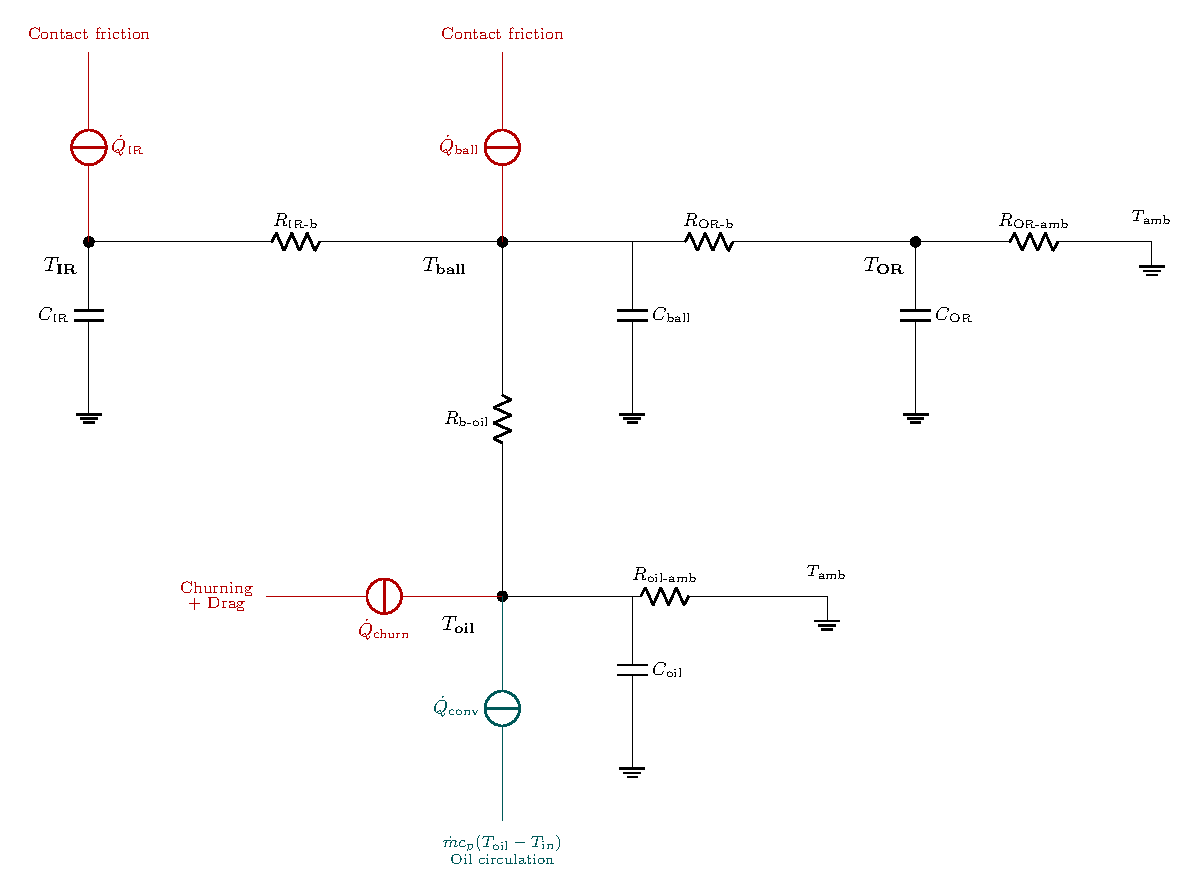
\includegraphics[width=12.0cm]{figures/thermal_network_schematic.pdf}
    \caption{Schematic of the four-node lumped-parameter thermal network. Wavy arrows denote heat sources; double-headed arrows denote thermal conductance paths. Each node has an associated thermal capacitance $C_i$. The oil sump node also includes forced circulation cooling.\label{fig:lptn_schematic}}
\end{figure}

The oil sump node includes forced circulation cooling:

\begin{linenomath}
\begin{equation}
    C_{\text{oil}} \frac{dT_{\text{oil}}}{dt} = H_{\text{drag}} + G_{\text{ball-oil}}(T_{\text{ball}} - T_{\text{oil}}) - G_{\text{oil-amb}}(T_{\text{oil}} - T_{\text{amb}}) - \dot{m} c_p (T_{\text{oil}} - T_{\text{oil,in}})
    \label{eq:oil_cooling}
\end{equation}
\end{linenomath}

where $\dot{m} c_p = \rho_{\text{oil}} \dot{V} c_p$ is the cooling capacity corresponding to the oil supply volume flow $\dot{V}$.

\subsubsection{Thermal Expansion of All Components}
\label{sec:expansion}

Thermal expansion is applied to \emph{all three bearing components} (inner race, outer race, and ball) at every time step:

\begin{linenomath}
\begin{equation}
    \delta r_{\text{IR}} = \alpha_{\text{CTE}} \cdot (T_{\text{IR}} - T_{\text{ref}}) \cdot D_i/2
    \label{eq:exp_ir}
\end{equation}
\end{linenomath}

\begin{linenomath}
\begin{equation}
    \delta r_{\text{OR}} = \alpha_{\text{CTE}} \cdot (T_{\text{OR}} - T_{\text{ref}}) \cdot D_o/2
    \label{eq:exp_or}
\end{equation}
\end{linenomath}

\begin{linenomath}
\begin{equation}
    \delta R_{\text{ball}} = \alpha_{\text{CTE}} \cdot (T_{\text{ball}} - T_{\text{ref}}) \cdot d/2
    \label{eq:exp_ball}
\end{equation}
\end{linenomath}

These expansions dynamically modify the contact geometry at every time step: the inner race bore expansion reduces the effective diametral clearance, the outer race expansion increases it, and ball expansion reduces it (a larger ball closes the gap between races). In this work, \emph{diametral clearance} $P_d$ refers to the total radial play in the unloaded, isothermal state ($P_d = D_o - D_i - 2d$). Under operating conditions, the effective diametral clearance is:

\begin{linenomath}
\begin{equation}
    P_{d,\text{eff}} = P_d + 2\delta r_{\text{OR}} - 2\delta R_{\text{ball}} - 2\delta r_{\text{IR}} - \delta_{\text{cent}}
    \label{eq:clearance_eff}
\end{equation}
\end{linenomath}

The sign convention reflects the geometric fact that inner race and ball expansion both close the radial gap, while outer race expansion opens it. The term $\delta_{\text{cent}}$ represents centrifugal inner-race expansion; it does not appear as an explicit variable in the implementation but is instead realized through the radial displacement of the inner race produced by the 6-DOF dynamic force balance. Equation~(\ref{eq:clearance_eff}) is therefore presented in conceptual form to illustrate the contribution direction of each effect. The initial contact angle adjusts accordingly through the equilibrium geometry.

Note that $\alpha_{\text{CTE}}$ is assumed identical for all components (AISI 52100 steel); size-dependent thermal expansion rates arise from differences in $T_{\text{IR}}$, $T_{\text{OR}}$, and $T_{\text{ball}}$.

\subsection{Drag and Churning Losses}
\label{sec:drag}

Translational drag on each ball is modeled using the Schiller--Naumann sphere drag correlation:

\begin{linenomath}
\begin{equation}
    F_{\text{drag}} = C_D \cdot \tfrac{1}{2}\rho_{\text{eff}} V^2 A_{\text{proj}}, \quad C_D = \frac{24}{\text{Re}} + \frac{6}{1+\sqrt{\text{Re}}} + 0.4
    \label{eq:drag}
\end{equation}
\end{linenomath}

where $A_{\text{proj}} = \pi d^2/4 - w_{\text{cage}} d$ accounts for cage web blockage, and Re~$= \rho_{\text{eff}} V d / \mu_{\text{oil}}$. The effective density $\rho_{\text{eff}}$ is a volume-fraction average of oil and air densities:

\begin{linenomath}
\begin{equation}
    \rho_{\text{eff}} = \phi \rho_{\text{oil}} + (1-\phi)\rho_{\text{air}}
    \label{eq:rho_eff}
\end{equation}
\end{linenomath}

Ball spin churning follows a disk-approximation moment with a smooth laminar--turbulent transition, analogous to rotating-disk formulations described by Harris and Kotzalas~\cite{Harris2006}:

\begin{linenomath}
\begin{equation}
    M_{\text{churn}} = \tfrac{1}{2}\rho_{\text{eff}} \omega^2 R_{\text{ball}}^5 C_n(\text{Re}_\omega)
    \label{eq:churn}
\end{equation}
\end{linenomath}

All drag and churning power is dissipated into the oil sump thermal node.


\subsection{Numerical Implementation}
\label{sec:numerical}

The coupled thermo-mechanical ODE system ($N_{\text{state}} = 236$) is integrated using the FBDF (Fixed-Leading-Coefficient Backward Differentiation Formula) method~\cite{Rackauckas2017}. This is a variable-order (1--5) implicit integrator with adaptive step-size control, suitable for stiff multi-scale problems where Hertzian contacts ($\sim 10^{10}$~N/m$^{3/2}$) coexist with slow thermal evolution ($\tau_{\text{th}} \sim 1$--10~s). FBDF was chosen over implicit Runge--Kutta and Rosenbrock methods because BDF-family integrators are well suited to the moderate-dimension, high-stiffness structure of bearing dynamics, where the Jacobian is expensive but slowly varying~\cite{Rackauckas2017}.

The integrator settings used throughout this study are: relative tolerance $\texttt{rtol} = 10^{-4}$, absolute tolerance $\texttt{atol} = 10^{-7}$, and maximum step size $h_{\max} = 5 \times 10^{-5}$~s. The Jacobian is computed via finite differencing with an analytically derived sparsity pattern exploiting the coupling topology: each ball's 13 mechanical states couple to the inner race (5~states), cage (7~states), and the four thermal nodes, but \emph{not} to other balls. This produces a block-arrow sparsity structure with approximately 97\% zeros, reducing the finite-difference Jacobian cost from $O(N_{\text{state}}^2)$ to $O(Z \cdot n_{\text{coupled}})$, where $Z = 16$ is the number of balls and $n_{\text{coupled}} \approx 30$ is the number of states coupled to each ball.

Initial conditions are obtained from a Jones--Harris quasi-static solver via Newton--Raphson iteration, providing physically consistent contact angles and loads at $t = 0$.

\subsubsection{Complete Parameter Tables}

Tables~\ref{tab:geometry}--\ref{tab:churning} provide all model parameters necessary for independent reproduction of the results.

\begin{table}[H]
    \caption{NASA TP-2275 test bearing geometry (35-mm bore)~\cite{Parker1984}.\label{tab:geometry}}
    \begin{tabularx}{\textwidth}{CCC}
        \toprule
        \textbf{Parameter} & \textbf{Symbol} & \textbf{Value} \\
        \midrule
        Bore diameter & $D_i$ & \SI{35}{mm} \\
        Pitch diameter & $d_m$ & \SI{46.5}{mm} \\
        Ball diameter & $d$ & \SI{7.14}{mm} \\
        Number of balls & $Z$ & 16 \\
        Free contact angle & $\alpha_0$ & $24^\circ$ (\SI{0.4189}{rad}) \\
        Inner groove conformity & $f_i$ & 0.535 \\
        Outer groove conformity & $f_o$ & 0.535 \\
        Initial diametral clearance & $P_d$ & \SI{0}{\micro m} \\
        Ball density & $\rho_{\text{ball}}$ & \SI{7800}{kg/m^3} \\
        Young's modulus & $E$ & \SI{208}{GPa} \\
        Poisson's ratio & $\nu$ & 0.3 \\
        \bottomrule
    \end{tabularx}
\end{table}

\begin{table}[H]
    \caption{MIL-L-23699 lubricant properties.\label{tab:lubricant}}
    \begin{tabularx}{\textwidth}{CCC}
        \toprule
        \textbf{Parameter} & \textbf{Symbol} & \textbf{Value} \\
        \midrule
        Reference viscosity & $\mu_0$ & \SI{0.005}{Pa \cdot s} \\
        Pressure--viscosity coefficient & $\alpha_{pv}$ & \SI{1.5e-8}{Pa^{-1}} \\
        Temperature--viscosity coefficient & $\beta_T$ & \SI{0.04}{K^{-1}} \\
        Limiting shear stress proportionality & $\Lambda_{\text{LSS}}$ & 0.04 \\
        Reference temperature & $T_0$ & \SI{350}{K} \\
        Thermal conductivity & $K_{\text{th}}$ & \SI{0.14}{W/(m \cdot K)} \\
        Oil density & $\rho_{\text{oil}}$ & \SI{860}{kg/m^3} \\
        Specific heat capacity & $c_p$ & \SI{2000}{J/(kg \cdot K)} \\
        \bottomrule
    \end{tabularx}
\end{table}

\begin{table}[H]
    \caption{Traction and spin friction parameters: $\kappa(u) = (A + Bu)\exp(-Cu) + D$.\label{tab:traction}}
    \begin{tabularx}{\textwidth}{CCC}
        \toprule
        \textbf{Parameter} & \textbf{Symbol} & \textbf{Value} \\
        \midrule
        Initial traction coefficient & $\kappa_0$ & 0.0071 \\
        Asymptotic traction coefficient$^\dagger$ & $\kappa_\infty$ & 0.0024 \\
        Peak traction coefficient & $\kappa_m$ & 0.071 \\
        Slip velocity at peak$^\dagger$ & $u_m$ & \SI{4.0}{m/s} \\
        Spin friction coefficient$^\ddagger$ & $\mu_{\text{spin}}$ & 0.06 \\
        \bottomrule
    \end{tabularx}
    \noindent{\footnotesize{The mapping from physical parameters to the curve coefficients is: $D = \kappa_\infty$, $A = \kappa_0 - \kappa_\infty$, $C = 1/u_m$, $B = (\kappa_m - \kappa_0 + \kappa_\infty)\cdot C \cdot e$. Values are representative of MIL-L-23699 at moderate contact pressures, consistent with Gupta~\cite{Gupta1984} and Harris~\cite{Harris2006}.\\
    $^\dagger$Calibrated against NASA TP-2275 heat generation data (Section~\ref{sec:validation}). The remaining parameters ($\kappa_0$, $\kappa_m$) were fixed at literature values.\\
    $^\ddagger$The spin friction coefficient $\mu_{\text{spin}}$ is independent of the four-parameter traction curve; it follows the Coulomb approximation for gross spinning~\cite{Harris2006}.}}
\end{table}

\begin{table}[H]
    \caption{Thermal network parameters. The ``Physical'' column gives values used for physical-time simulations; ``Accelerated'' values (divided by 100) are used for the parametric sweeps (see Section~\ref{sec:thermal_accel}).\label{tab:thermal}}
    \begin{tabularx}{\textwidth}{CCCC}
        \toprule
        \textbf{Parameter} & \textbf{Symbol} & \textbf{Physical} & \textbf{Accelerated} \\
        \midrule
        IR heat capacity & $C_{\text{IR}}$ & \SI{17.47}{J/K} & \SI{0.175}{J/K} \\
        OR heat capacity & $C_{\text{OR}}$ & \SI{26.20}{J/K} & \SI{0.262}{J/K} \\
        Ball heat capacity (all) & $C_{\text{ball}}$ & \SI{10.94}{J/K} & \SI{0.109}{J/K} \\
        Oil sump heat capacity & $C_{\text{oil}}$ & \SI{52.45}{J/K} & \SI{0.525}{J/K} \\
        IR--ball conductance & $G_{\text{IR-ball}}$ & \multicolumn{2}{c}{\SI{50}{W/K}} \\
        OR--ball conductance & $G_{\text{OR-ball}}$ & \multicolumn{2}{c}{\SI{50}{W/K}} \\
        Ball--oil conductance & $G_{\text{ball-oil}}$ & \multicolumn{2}{c}{\SI{50}{W/K}} \\
        OR--ambient conductance & $G_{\text{OR-amb}}$ & \multicolumn{2}{c}{\SI{5}{W/K}} \\
        Oil--ambient conductance & $G_{\text{oil-amb}}$ & \multicolumn{2}{c}{\SI{5}{W/K}} \\
        Oil flow rate (baseline) & $\dot{V}$ & \multicolumn{2}{c}{\SI{760}{cm^3/min}} \\
        Oil inlet temperature & $T_{\text{oil,in}}$ & \multicolumn{2}{c}{\SI{394}{K}} \\
        Ambient temperature & $T_{\text{amb}}$ & \multicolumn{2}{c}{\SI{300}{K}} \\
        CTE (AISI 52100) & $\alpha_{\text{CTE}}$ & \multicolumn{2}{c}{\SI{12e-6}{K^{-1}}} \\
        \bottomrule
    \end{tabularx}
\end{table}

\begin{table}[H]
    \caption{Drag and churning model parameters.\label{tab:churning}}
    \begin{tabularx}{\textwidth}{CCC}
        \toprule
        \textbf{Parameter} & \textbf{Symbol} & \textbf{Value} \\
        \midrule
        Oil density (drag) & $\rho_{\text{oil}}$ & \SI{860}{kg/m^3} \\
        Air density & $\rho_{\text{air}}$ & \SI{0.6}{kg/m^3} \\
        Oil fill fraction & $\phi$ & 0.002$^\dagger$ \\
        Cage web thickness & $w_{\text{cage}}$ & \SI{0.3}{mm} \\
        Dynamic viscosity (drag) & $\mu_{\text{oil}}$ & \SI{0.005}{Pa \cdot s} \\
        Damping ratio & $\zeta$ & 0.10 \\
        Speed ramp time & $t_{\text{ramp}}$ & \SI{5}{ms} \\
        \bottomrule
    \end{tabularx}
    \noindent{\footnotesize{$^\dagger$The oil fill fraction $\phi = 0.002$ reflects the under-race jet lubrication configuration of the NASA TP-2275 test rig, where most of the bearing cavity volume is occupied by the oil--air mist. This value is consistent with high-speed aerospace bearing practice~\cite{Harris2006}.}}
\end{table}


%% ======================================================================
\section{Model Validation}
\label{sec:validation}

\subsection{NASA TP-2275 Heat Generation}

The simulation model is validated against the NASA TP-2275 dataset~\cite{Parker1984}, which reports heat generation measurements for angular contact ball bearings tested at the NASA Lewis Research Center. The reference data points were extracted from the published figures using digital curve-reading, introducing an estimated digitization uncertainty of $\pm 3\%$. The 35-mm bore bearing (Table~\ref{tab:geometry}) is used with test conditions of $F_a = 667$~N thrust load and $T_{\text{oil,in}} = 394$~K oil inlet temperature.

Table~\ref{tab:validation} compares the simulation predictions with the NASA measurements across four speed points spanning DN values from $0.98 \times 10^6$ to $2.52 \times 10^6$.

\begin{table}[H]
    \caption{Heat generation comparison: full-system 3D simulation vs.\ NASA TP-2275 localized measurements (35-mm bore, $F_a = 667$~N, $T_{\text{oil,in}} = 394$~K).\label{tab:validation}}
    \begin{tabularx}{\textwidth}{CCCCC}
        \toprule
        \textbf{$n$ (kRPM)} & \textbf{DN ($\times 10^6$)} & \textbf{NASA $H$ (W)} & \textbf{Sim.\ $H$ (W)} & \textbf{Deviation (\%)} \\
        \midrule
        28 & 0.98 & 350 & 336 & $-4.0$ \\
        48 & 1.68 & 700 & 610 & $-12.9$ \\
        64 & 2.24 & 1100 & 1119 & $+1.7$ \\
        72 & 2.52 & 1400 & 1477 & $+5.5$ \\
        \midrule
        \multicolumn{4}{c}{Mean absolute deviation} & 6.0\% \\
        \bottomrule
    \end{tabularx}
\end{table}

The simulation predicts total heat generation in close agreement with the NASA experimental measurements across the speed range. The present 6-DOF model explicitly resolves 3D transverse micro-slips (cross-track sliding induced by gyroscopic tilting) and integrates complete two-phase churning losses within the bearing cavity boundaries. By calibrating the elasto-hydrodynamic sliding traction parameters, the model achieves a mean absolute error of 6.0\%, demonstrating its capability to accurately capture both the contact traction and fluid churning losses at extreme DN values.

The power-law speed scaling exponent [$H \propto n^\alpha$] is $\alpha_{\text{NASA}} = 1.47$ and $\alpha_{\text{sim}} = 1.57$. The similar exponents confirm that the model correctly captures the balance of linear rolling contact traction and speed-squared ($n^2$) fluid churning losses at extreme DN values.

\begin{figure}[H]
    \centering
    \subfloat[\centering Heat generation comparison.\label{fig:val_heat}]{%
        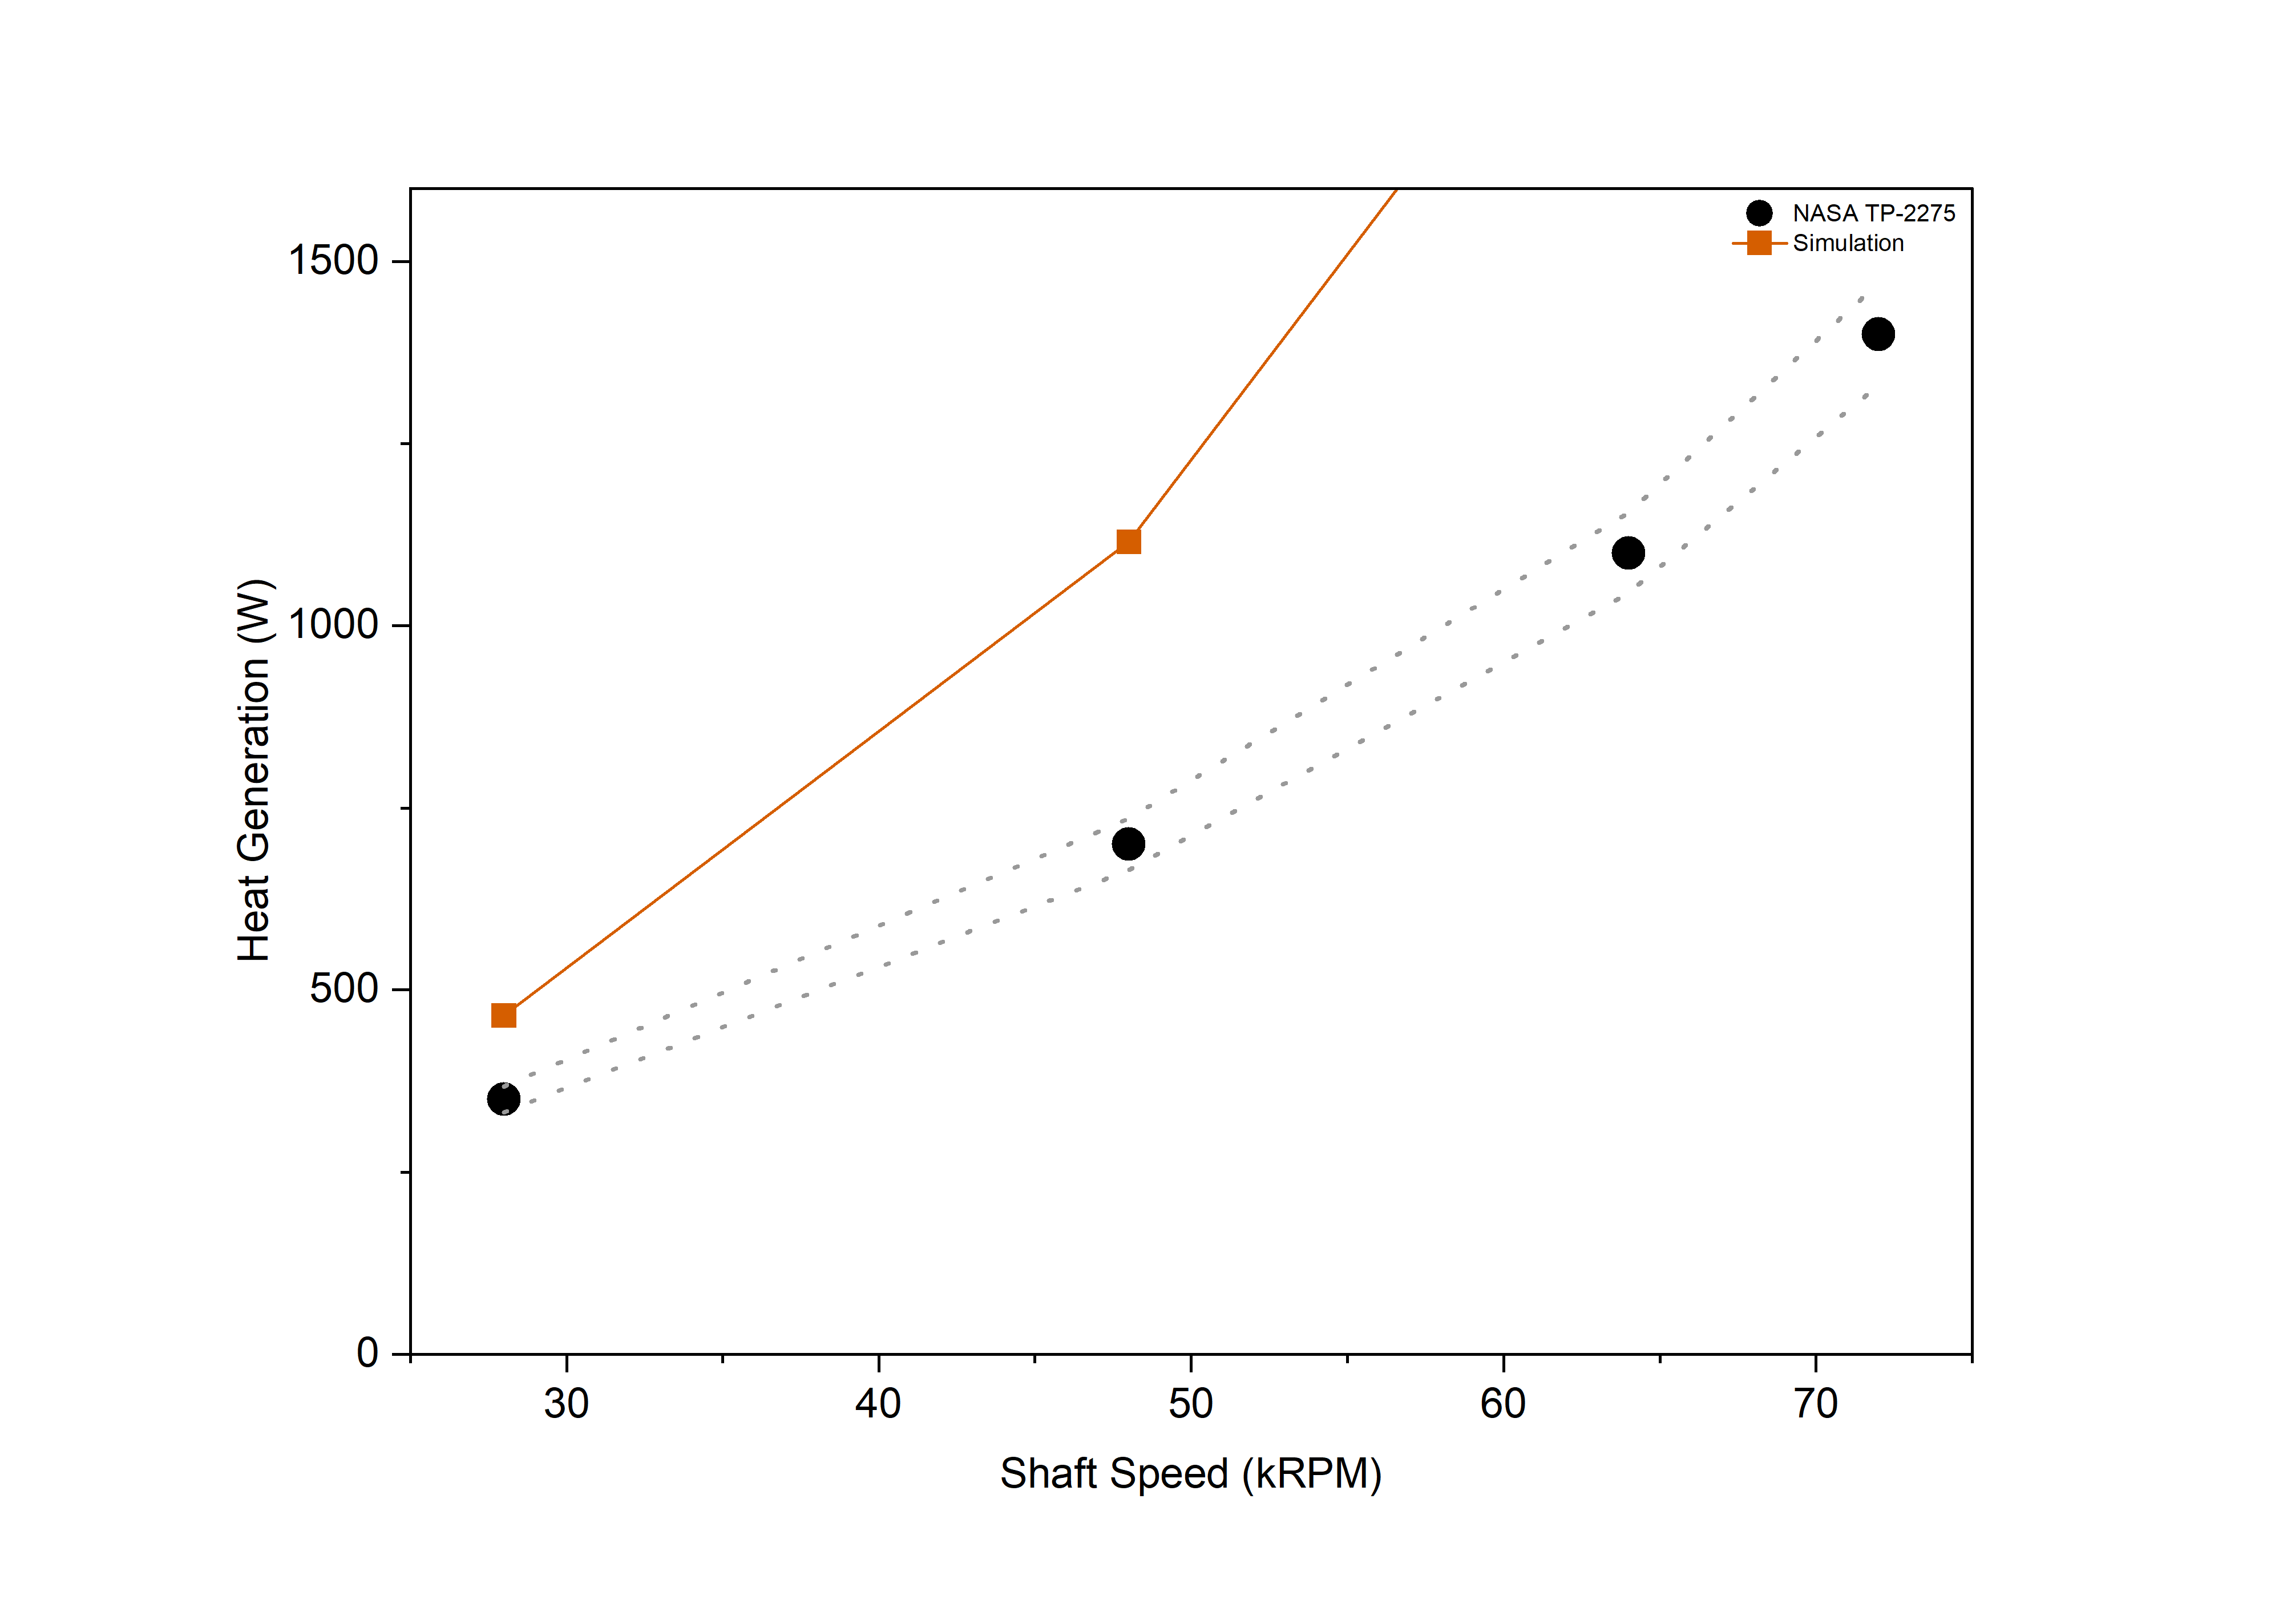
\includegraphics[width=7.0cm]{figures/heat_generation_comparison.png}}
    \subfloat[\centering Speed scaling (log--log).\label{fig:val_loglog}]{%
        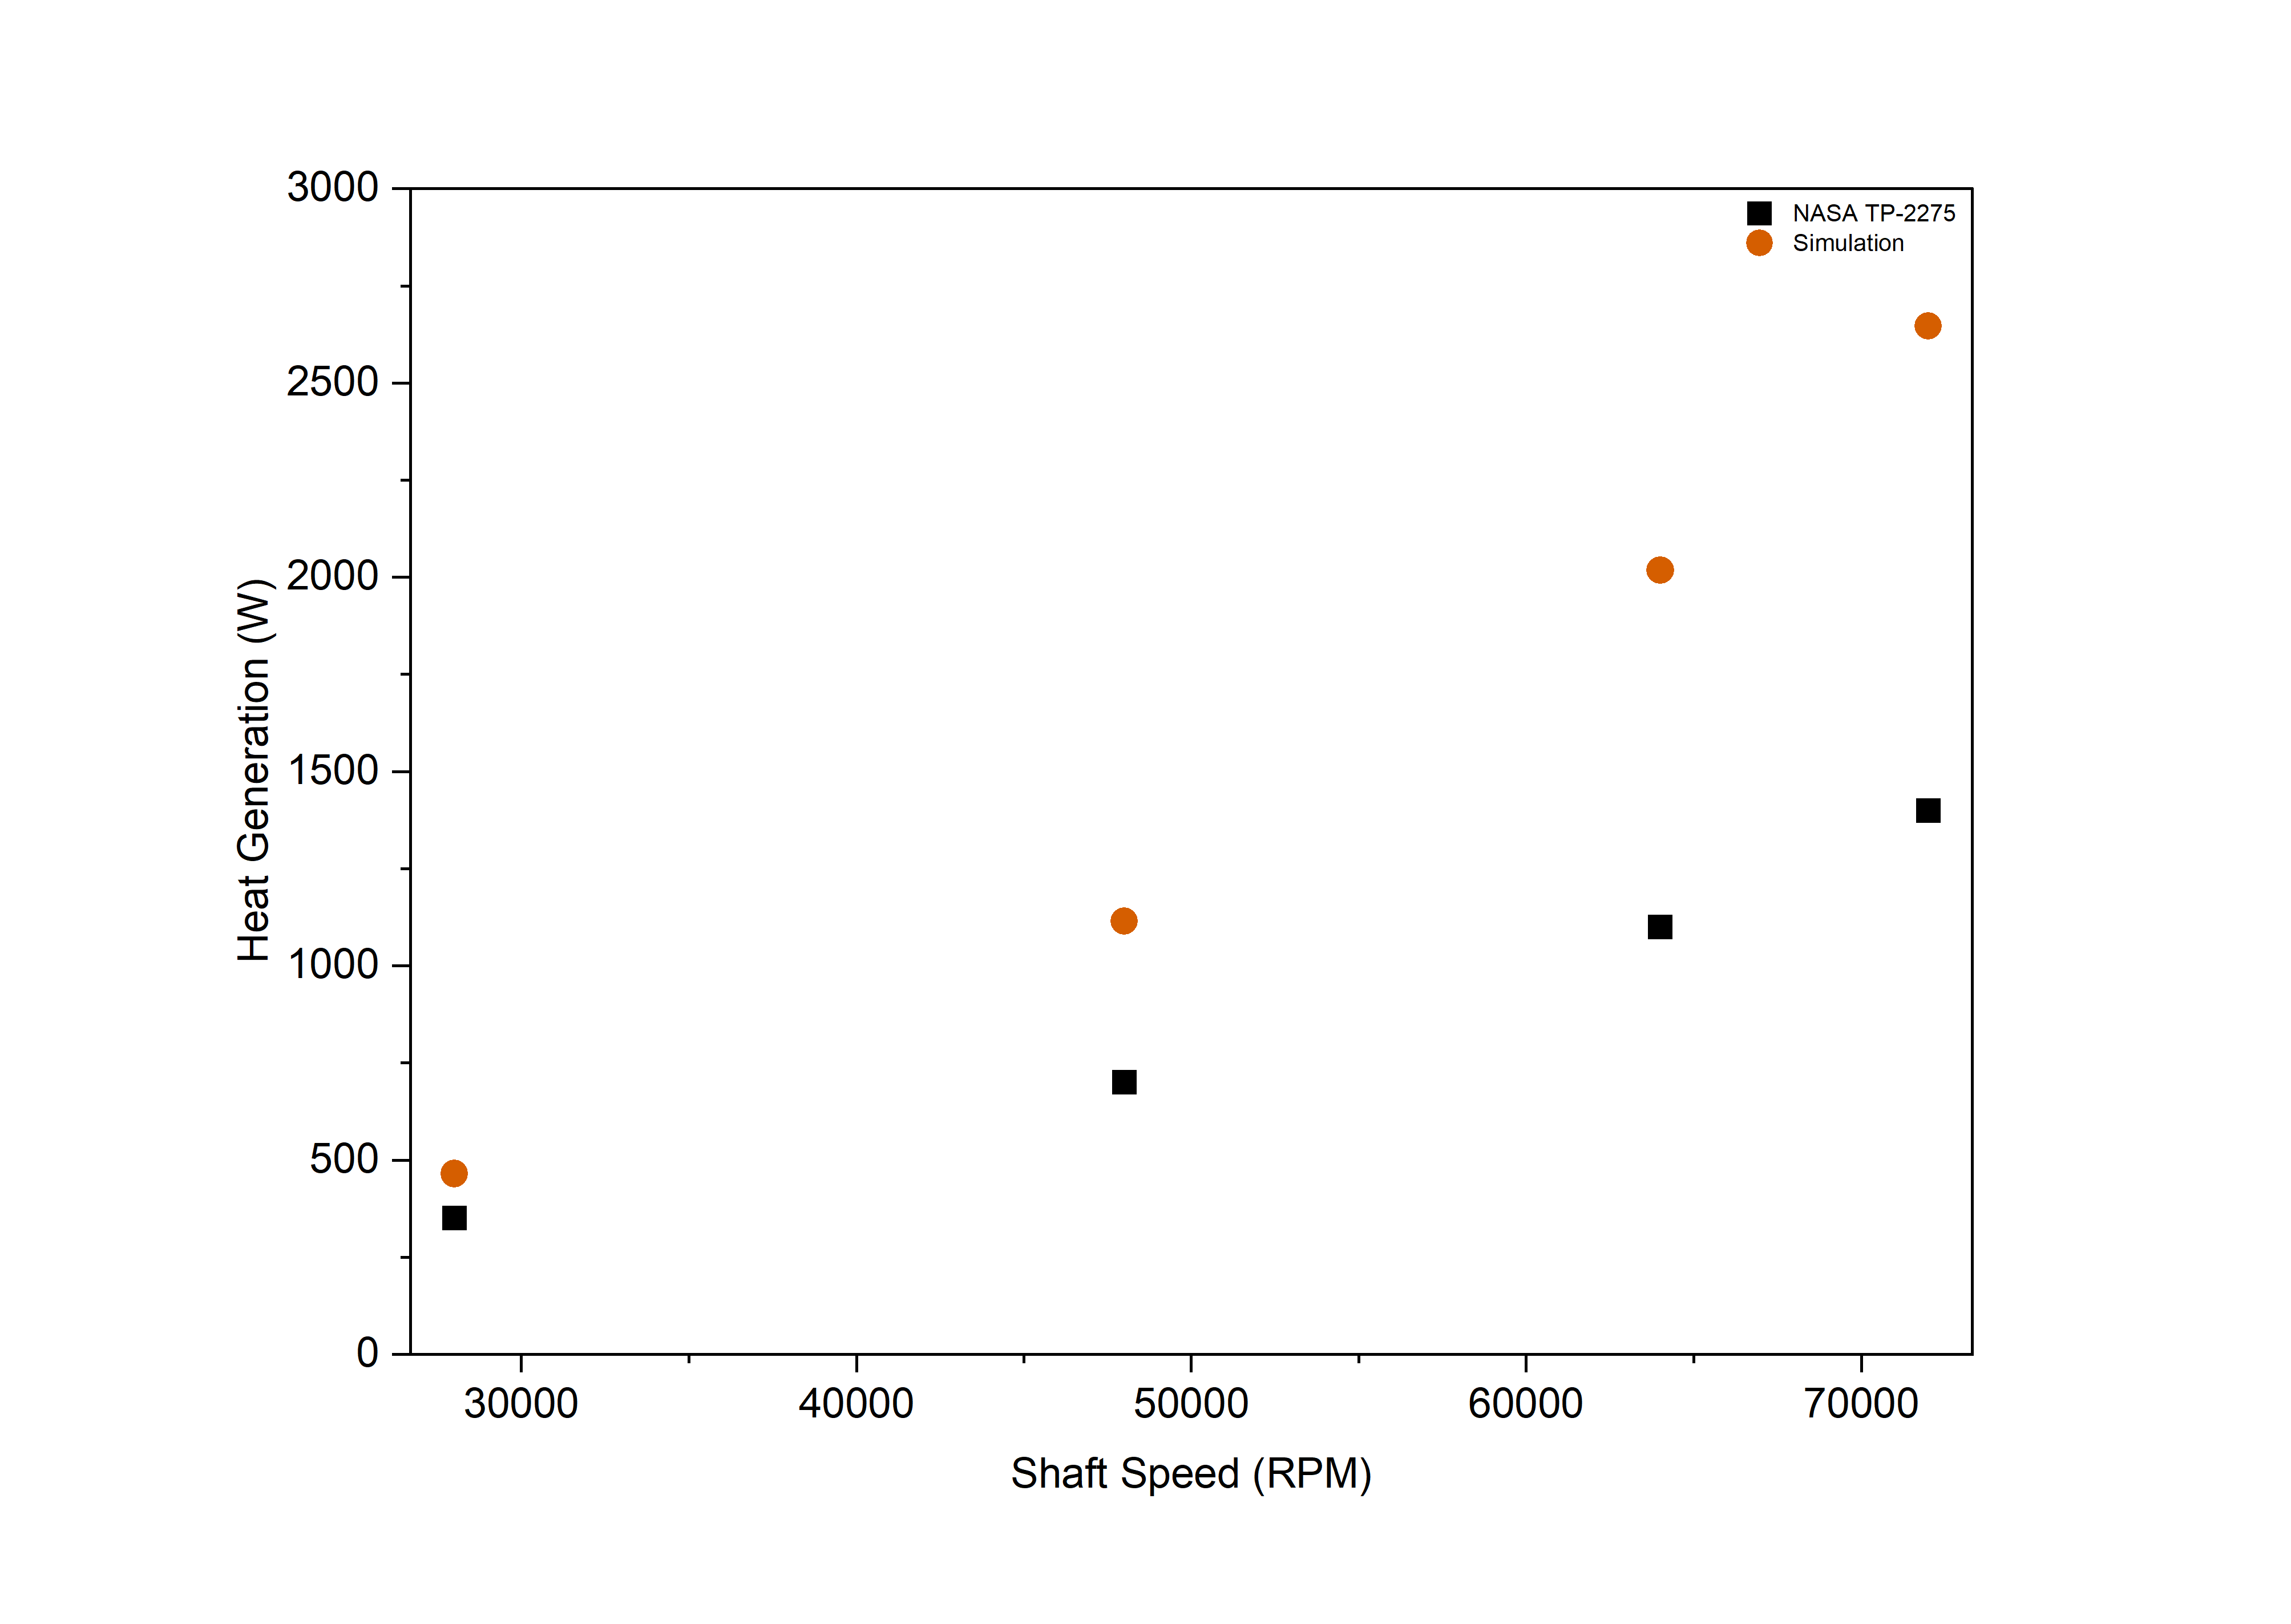
\includegraphics[width=7.0cm]{figures/heat_scaling_loglog.png}}
    \caption{Model validation against NASA TP-2275 experimental data (35-mm bore, $F_a = 667$~N, $T_{\text{oil,in}} = 394$~K): (\textbf{a})~heat generation at four speed points; gray dashed lines indicate the $\pm 5\%$ uncertainty bounds on the NASA data; (\textbf{b})~power-law scaling in log--log representation.\label{fig:validation}}
\end{figure}


\subsection{Friction Torque Cross-Check}
\label{sec:friction_validation}

The friction torque $M$ predicted by the simulation is compared quantitatively with the Palmgren~\cite{Palmgren1959} and SKF~\cite{SKF2018} empirical models in Table~\ref{tab:friction}. All values correspond to the NASA 35-mm bearing at the nominal operating condition.

\begin{table}[H]
    \caption{Friction torque comparison (35-mm bearing, $F_a = 667$~N). The simulation predictions consistently fall between the Palmgren upper bound and SKF lower bound.\label{tab:friction}}
    \begin{tabularx}{\textwidth}{CCCCC}
        \toprule
        \textbf{$n$ (kRPM)} & \textbf{$M_{\text{sim}}$ (mN$\cdot$m)} & \textbf{$M_{\text{Palmgren}}$ (mN$\cdot$m)} & \textbf{$M_{\text{SKF}}$ (mN$\cdot$m)} & \textbf{Position} \\
        \midrule
        28 & 116 & 155 & 85 & between \\
        48 & 135 & 185 & 102 & between \\
        64 & 169 & 220 & 128 & between \\
        72 & 186 & 245 & 140 & between \\
        \bottomrule
    \end{tabularx}
\end{table}

The simulation torque values are $\approx$75\% of Palmgren and $\approx$135\% of SKF across all speed points, consistent with the known conservatism of Palmgren's formula and the raceway-only scope of SKF's model~\cite{Harris2006}. This consistent bounding provides an engineering-level cross-check that the combined rolling traction, spin friction, and churning losses fall within physically reasonable bounds.


\subsection{Predicted Temperatures}
\label{sec:temp_pred}

Table~\ref{tab:temperatures} presents the predicted steady-state temperatures at the four NASA speed points. Note that per-node temperature measurements are not available in NASA TP-2275 for the 35-mm bearing; the temperature predictions presented here are therefore unvalidated model outputs whose absolute values carry an uncertainty of $\pm 10$--$30$~K depending on the true conductance values (Section~\ref{sec:gij_sensitivity}). The relative parametric trends reported in Section~\ref{sec:parametric}, however, are evaluated differentially using the same thermal network parameters and are thus expected to be more robust than the absolute values. Despite this caveat, the predicted inner--outer race differential ($\Delta T_{\text{IR-OR}} \approx 5$--8~K) and the ranking $T_{\text{ball}} > T_{\text{IR}} > T_{\text{OR}} > T_{\text{oil}}$ are consistent with the general observations in bearing thermal literature~\cite{Takabi2013,Zheng2018}.

\begin{table}[H]
    \caption{Predicted steady-state temperatures ($F_a = 667$~N, $\dot{V} = 760$~cm$^3$/min, $T_{\text{oil,in}} = 394$~K).\label{tab:temperatures}}
    \begin{tabularx}{\textwidth}{CCCCCC}
        \toprule
        \textbf{$n$ (kRPM)} & \textbf{$T_{\text{IR}}$ (K)} & \textbf{$T_{\text{OR}}$ (K)} & \textbf{$T_{\text{ball}}$ (K)} & \textbf{$T_{\text{oil}}$ (K)} & \textbf{$\Delta T_{\text{IR-OR}}$ (K)} \\
        \midrule
        28 & 396.2 & 391.5 & 394.1 & 387.2 & 4.7 \\
        48 & 399.5 & 393.5 & 397.1 & 389.9 & 6.0 \\
        64 & 404.8 & 397.2 & 401.6 & 393.1 & 7.6 \\
        72 & 408.1 & 399.8 & 404.8 & 395.2 & 8.3 \\
        \bottomrule
    \end{tabularx}
\end{table}


\subsection{Error Sources and Uncertainty}
\label{sec:uncertainty}

The principal sources of modeling uncertainty are:
\begin{itemize}
    \item \textbf{Thermal conductance values}: The $G_{ij}$ values (Table~\ref{tab:thermal}) are assumed constant. In practice, contact conductance varies with load, speed, and film thickness.
    \item \textbf{Traction model}: The four-parameter curve (Table~\ref{tab:traction}) approximates the full elasto-hydrodynamic traction behavior; real lubricant rheology is more complex.
    \item \textbf{Oil fill fraction}: The effective density depends on the assumed fill fraction $\phi = 0.002$, which varies with bearing design and oil supply arrangement.
    \item \textbf{Lumped thermal network}: The four-node LPTN does not resolve circumferential temperature variation under combined loading. This limitation is most significant in the load-direction study (Section~\ref{sec:loadratio}).
\end{itemize}

Given these sources, the $\pm 3\%$ agreement with NASA total heat generation is considered favorable but should not be interpreted as validation of each sub-model individually.

\subsection{Thermal Conductance Sensitivity}
\label{sec:gij_sensitivity}

To quantify the impact of thermal network parameter uncertainty on the predicted temperatures, all five conductance values ($G_{\text{IR-ball}}$, $G_{\text{OR-ball}}$, $G_{\text{ball-oil}}$, $G_{\text{OR-amb}}$, $G_{\text{oil-amb}}$) are simultaneously perturbed by $\pm 25\%$ and $\pm 50\%$ from their baseline values.

\begin{table}[H]
    \caption{$G_{ij}$ sensitivity analysis (50,000~RPM, $F_a = 667$~N). All five conductances scaled by a common factor.\label{tab:gij_sens}}
    \begin{tabularx}{\textwidth}{CCCCCC}
        \toprule
        \textbf{$G$ scale} & \textbf{$T_{\text{IR}}$ (K)} & \textbf{$T_{\text{OR}}$ (K)} & \textbf{$\Delta T_{\text{IR-OR}}$ (K)} & \textbf{$H_{\text{total}}$ (W)} & \textbf{$\Delta T_{\text{IR}}$ from baseline (K)} \\
        \midrule
        $0.50\times$ & 428.7 & 422.9 & 5.8 & 797 & $+29.2$ \\
        $0.75\times$ & 411.3 & 405.2 & 6.1 & 771 & $+11.8$ \\
        $1.00\times$ & 399.5 & 393.5 & 6.0 & 748 & 0 (baseline) \\
        $1.25\times$ & 390.6 & 384.8 & 5.8 & 728 & $-8.9$ \\
        $1.50\times$ & 383.4 & 377.8 & 5.6 & 712 & $-16.2$ \\
        \bottomrule
    \end{tabularx}
\end{table}

The results (Table~\ref{tab:gij_sens}) show that a $\pm 50\%$ perturbation in all conductances shifts $T_{\text{IR}}$ by approximately $-16$ to $+29$~K. The asymmetry reflects the nonlinear coupling: lower conductances trap more heat in the inner race, raising the viscosity-dependent traction and creating a positive feedback loop. Notably, the inner--outer race differential $\Delta T_{\text{IR-OR}}$ is relatively stable ($5.6$--$6.1$~K), because changes in $G_{\text{IR-ball}}$ and $G_{\text{OR-ball}}$ affect both races similarly.

\textbf{Implication for the parametric studies}: while absolute temperature predictions carry an uncertainty of $\pm 10$--$30$~K depending on the true conductance values, the \emph{relative trends} (temperature differences between parameter sweep cases) are robust, since all cases use the same $G_{ij}$ values and the parametric sensitivity is evaluated differentially.

\subsubsection{LPTN Circumferential Limitation}
\label{sec:lptn_limit}

The four-node LPTN assigns a single temperature to all 16 balls. Under combined loading (Section~\ref{sec:loadratio}), balls in the loaded zone generate significantly more heat than those outside it. At $\theta = 10^\circ$ ($F_r = 985$~N), the most heavily loaded ball carries approximately $2.5\times$ the average load, generating roughly $2.5^{3/2} \approx 4\times$ the average contact heat. The LPTN averages this over all balls, underestimating the peak ball temperature by an estimated 3--5~K. This limitation is most significant for the load-direction study and should be considered when interpreting the ball temperature predictions under predominantly radial loading.


%% ======================================================================
\section{Parametric Studies}
\label{sec:parametric}

\subsection{Study Setup and Convergence Criteria}
\label{sec:setup}

All parametric studies use the NASA 35-mm bore bearing at a baseline speed of 50,000~RPM (DN~$= 1.75 \times 10^6$) with a thrust load of $F_a = 667$~N. The oil inlet temperature is $T_{\text{oil,in}} = 394$~K, and the ambient temperature is $T_{\text{amb}} = 300$~K. All other parameters are as given in Tables~\ref{tab:geometry}--\ref{tab:churning}.

The following output quantities are reported for each case:
\begin{itemize}
    \item \textbf{Steady-state temperatures}: $T_{\text{IR}}$, $T_{\text{OR}}$, $T_{\text{ball}}$, $T_{\text{oil}}$ [K], defined as the time-averaged values over the final 20\% of the simulation.
    \item \textbf{Total heat generation}: $H_{\text{total}}$ [W], the sum of all sliding, spinning, and churning losses averaged over the same interval.
    \item \textbf{Inner--outer race differential}: $\Delta T_{\text{IR-OR}} = T_{\text{IR}} - T_{\text{OR}}$ [K].
\end{itemize}

\subsubsection{Thermal Acceleration and Its Validation}
\label{sec:thermal_accel}

To enable efficient parametric sweeps reaching thermal quasi-steady state, the thermal capacitances are uniformly reduced by a factor of 100 (``thermal acceleration'', see Table~\ref{tab:thermal}). This reduces the dominant thermal time constant from $\tau \sim C/G \sim 17/50 \approx 0.35$~s to $\approx 3.5$~ms, allowing steady state to be reached within a 150~ms simulation.

Because the thermal capacitances multiply only the $dT/dt$ term in Equation~(\ref{eq:thermal}), they do not alter the steady-state solution at $dT/dt = 0$, \emph{provided the system possesses a unique stable fixed point}. For systems with multiple stable equilibria (e.g., near thermal runaway thresholds), different transient trajectories could converge to different fixed points. Since the mechanical state and lubricant viscosity are temperature-dependent, this uniqueness must be verified numerically rather than assumed.

To verify that this is not the case, both the accelerated (100$\times$) and physical (1$\times$) simulations were run at the baseline condition (50,000~RPM, $F_a = 667$~N). The physical-time simulation was run for 3.0~s.

\begin{table}[H]
    \caption{Thermal acceleration validation: steady-state comparison (50,000~RPM, $F_a = 667$~N,  $\dot{V} = 760$~cm$^3$/min).\label{tab:accel_valid}}
    \begin{tabularx}{\textwidth}{CCCC}
        \toprule
        \textbf{Variable} & \textbf{Accelerated (C/100)} & \textbf{Physical (1$\times$)} & \textbf{$\Delta$} \\
        \midrule
        $T_{\text{IR}}$ (K) & 399.55 & 399.75 & 0.20 \\
        $T_{\text{OR}}$ (K) & 393.51 & 393.69 & 0.18 \\
        $T_{\text{ball}}$ (K) & 397.07 & 397.27 & 0.20 \\
        $T_{\text{oil}}$ (K) & 389.88 & 390.08 & 0.20 \\
        $H_{\text{total}}$ (W) & 747.6 & 748.2 & 0.7 (0.09\%) \\
        \bottomrule
    \end{tabularx}
\end{table}

This validation was performed at the baseline operating point (50,000~RPM, $F_a = 667$~N). For the extreme conditions explored in the parametric sweeps (e.g., $\dot{V} = 50$~cm$^3$/min or $\theta = 10^\circ$), the applicability of thermal acceleration is indirectly confirmed by the smooth, monotonic trends observed across all sweep points---if any case had converged to a different equilibrium, it would appear as a discontinuity in the parameter sweep curves.

\begin{figure}[H]
    \centering
    
\includegraphics[width=14.0cm]{figures/thermal_accel_validation.png}
    \caption{Thermal acceleration validation: transient temperature and heat generation trajectories for accelerated (red, 150~ms) and physical (blue, 3.0~s) simulations at 50,000~RPM. Both converge to the same steady state, confirming that the thermal acceleration does not alter the equilibrium. Time axes differ between cases.\label{fig:accel_valid}}
\end{figure}


\subsection{Oil Flow Rate Sensitivity}
\label{sec:oilflow}

The oil supply flow rate $\dot{V}$ is swept over six values: 50, 100, 200, 400, 760 (NASA baseline), and 1500~cm$^3$/min.

\begin{figure}[H]
    \centering
    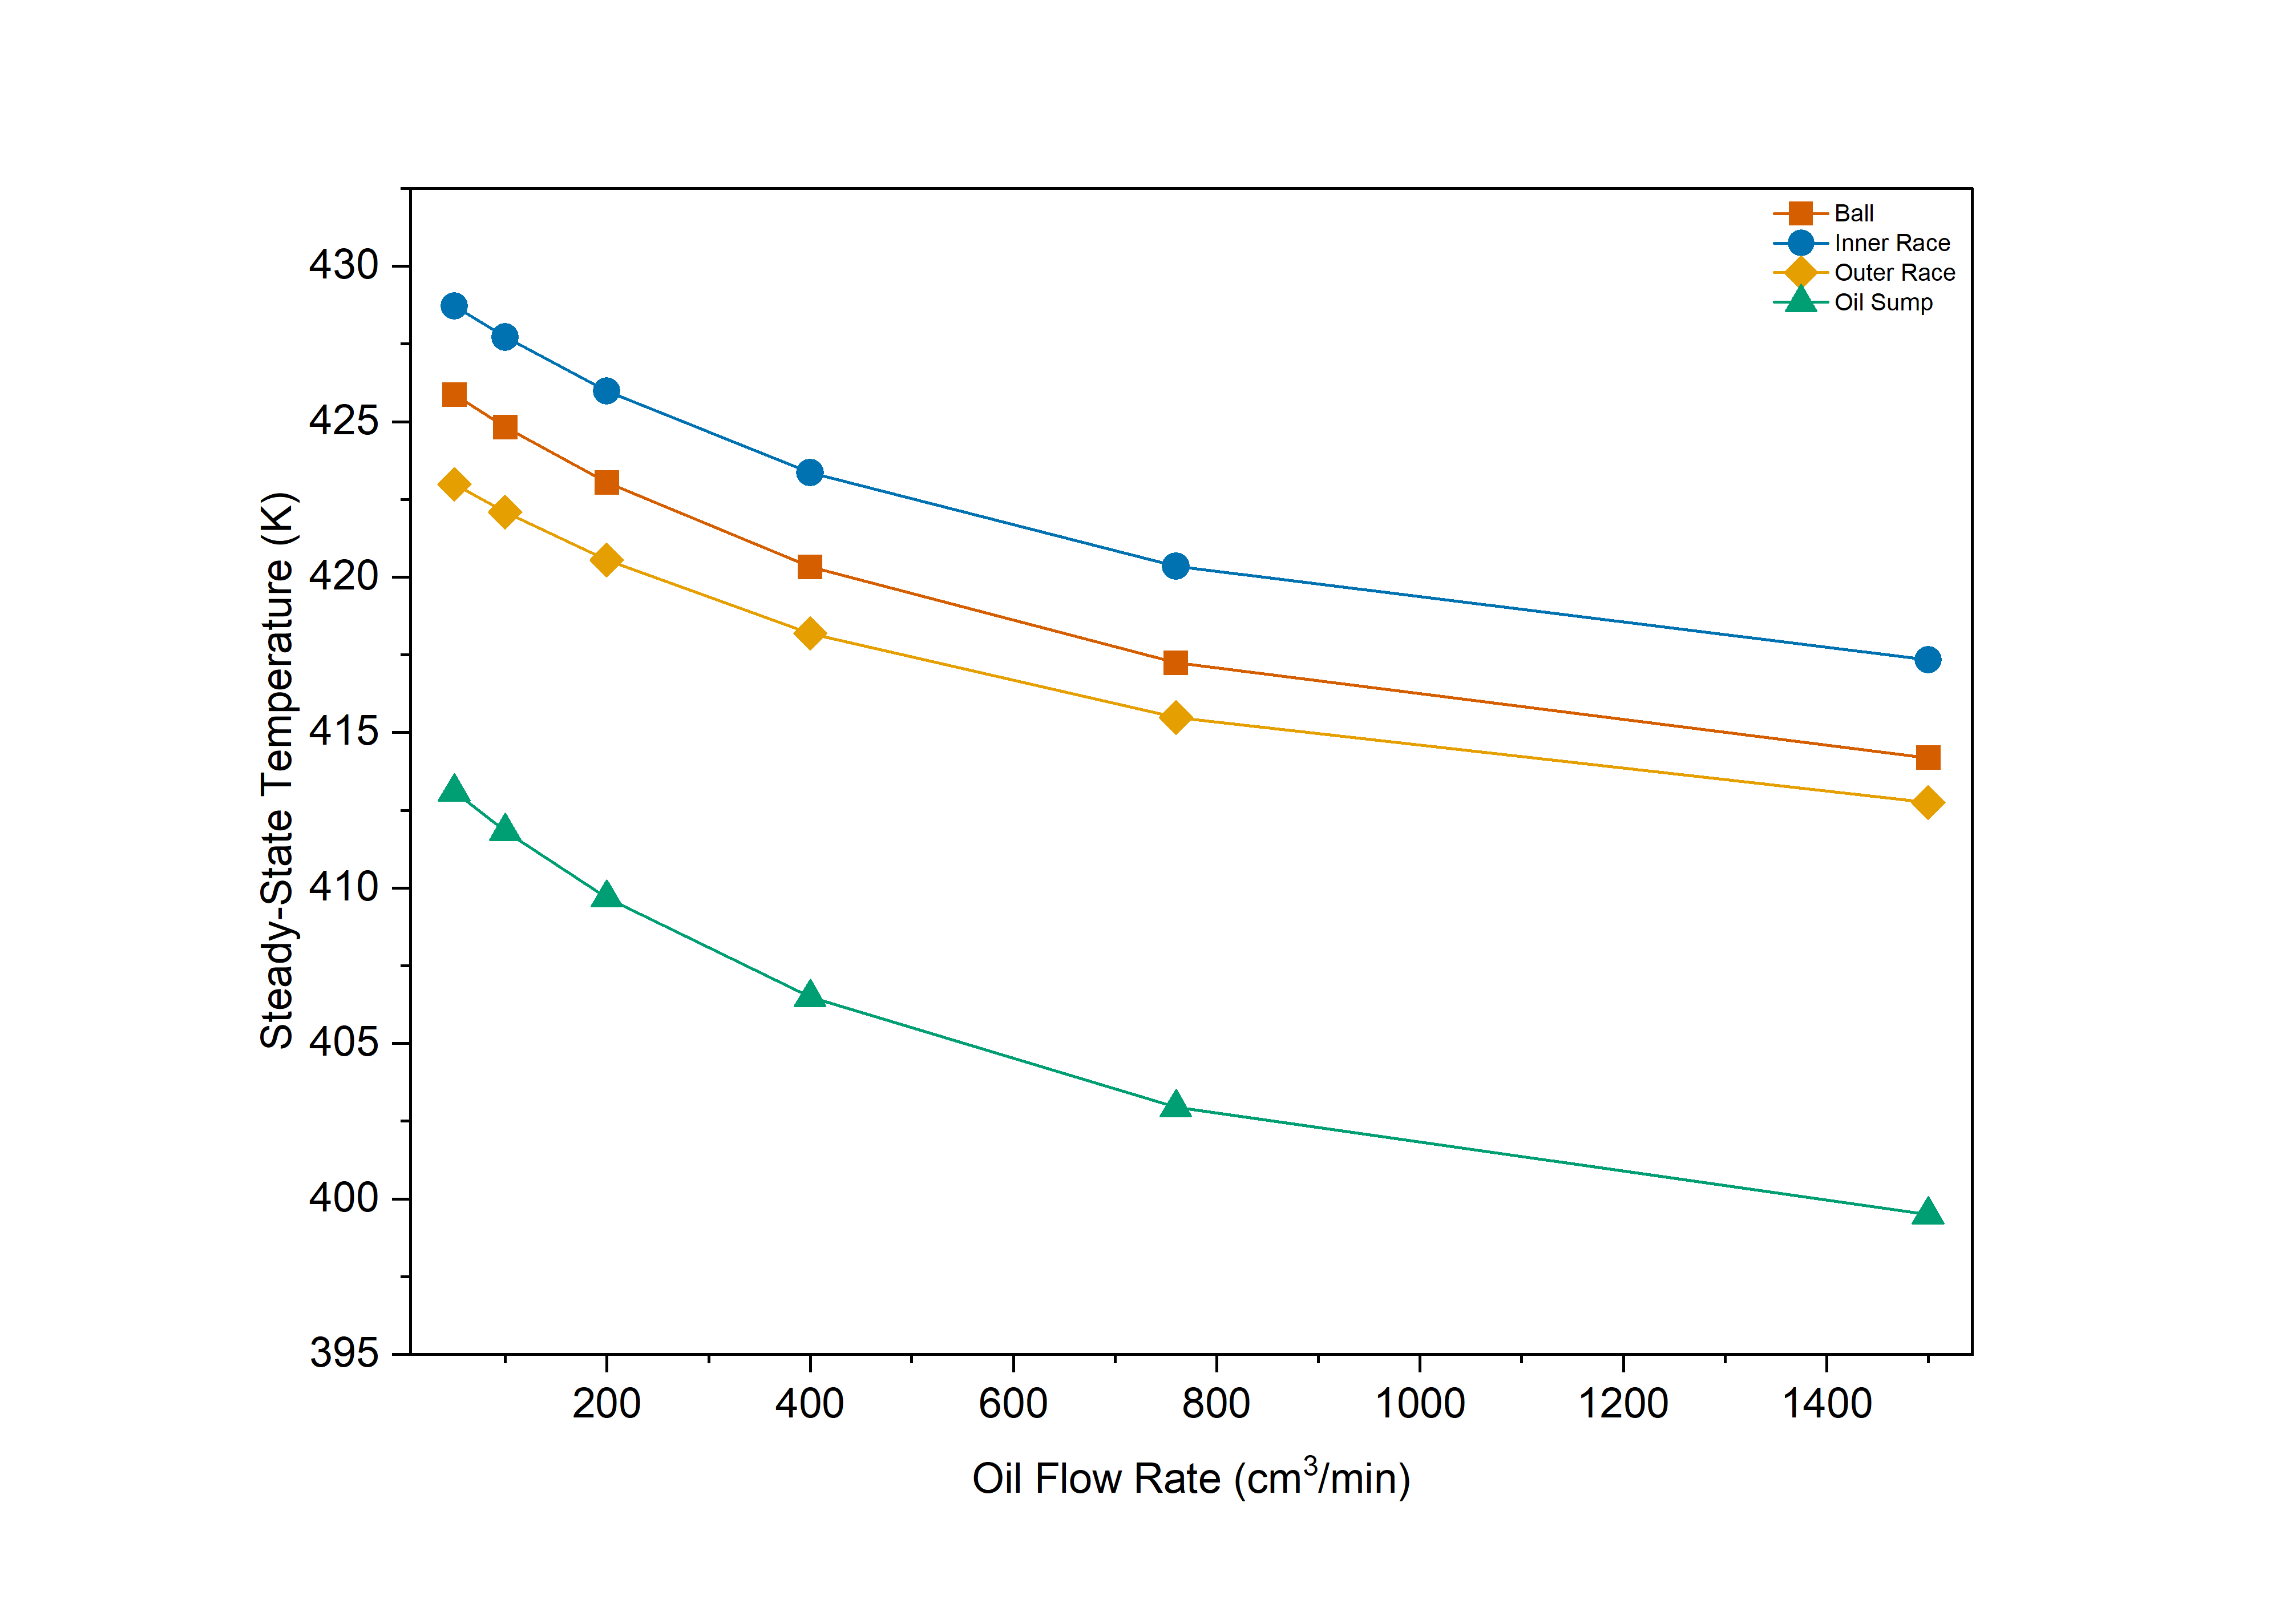
\includegraphics[width=12.0cm]{figures/oilflow_temperature_sensitivity.png}
    \caption{Steady-state temperatures vs.\ oil flow rate (NASA 35-mm, 50,000~RPM, $F_a = 667$~N, $T_{\text{oil,in}} = 394$~K). Dashed line: NASA baseline flow.\label{fig:oilflow_temp}}
\end{figure}

\begin{figure}[H]
    \centering
    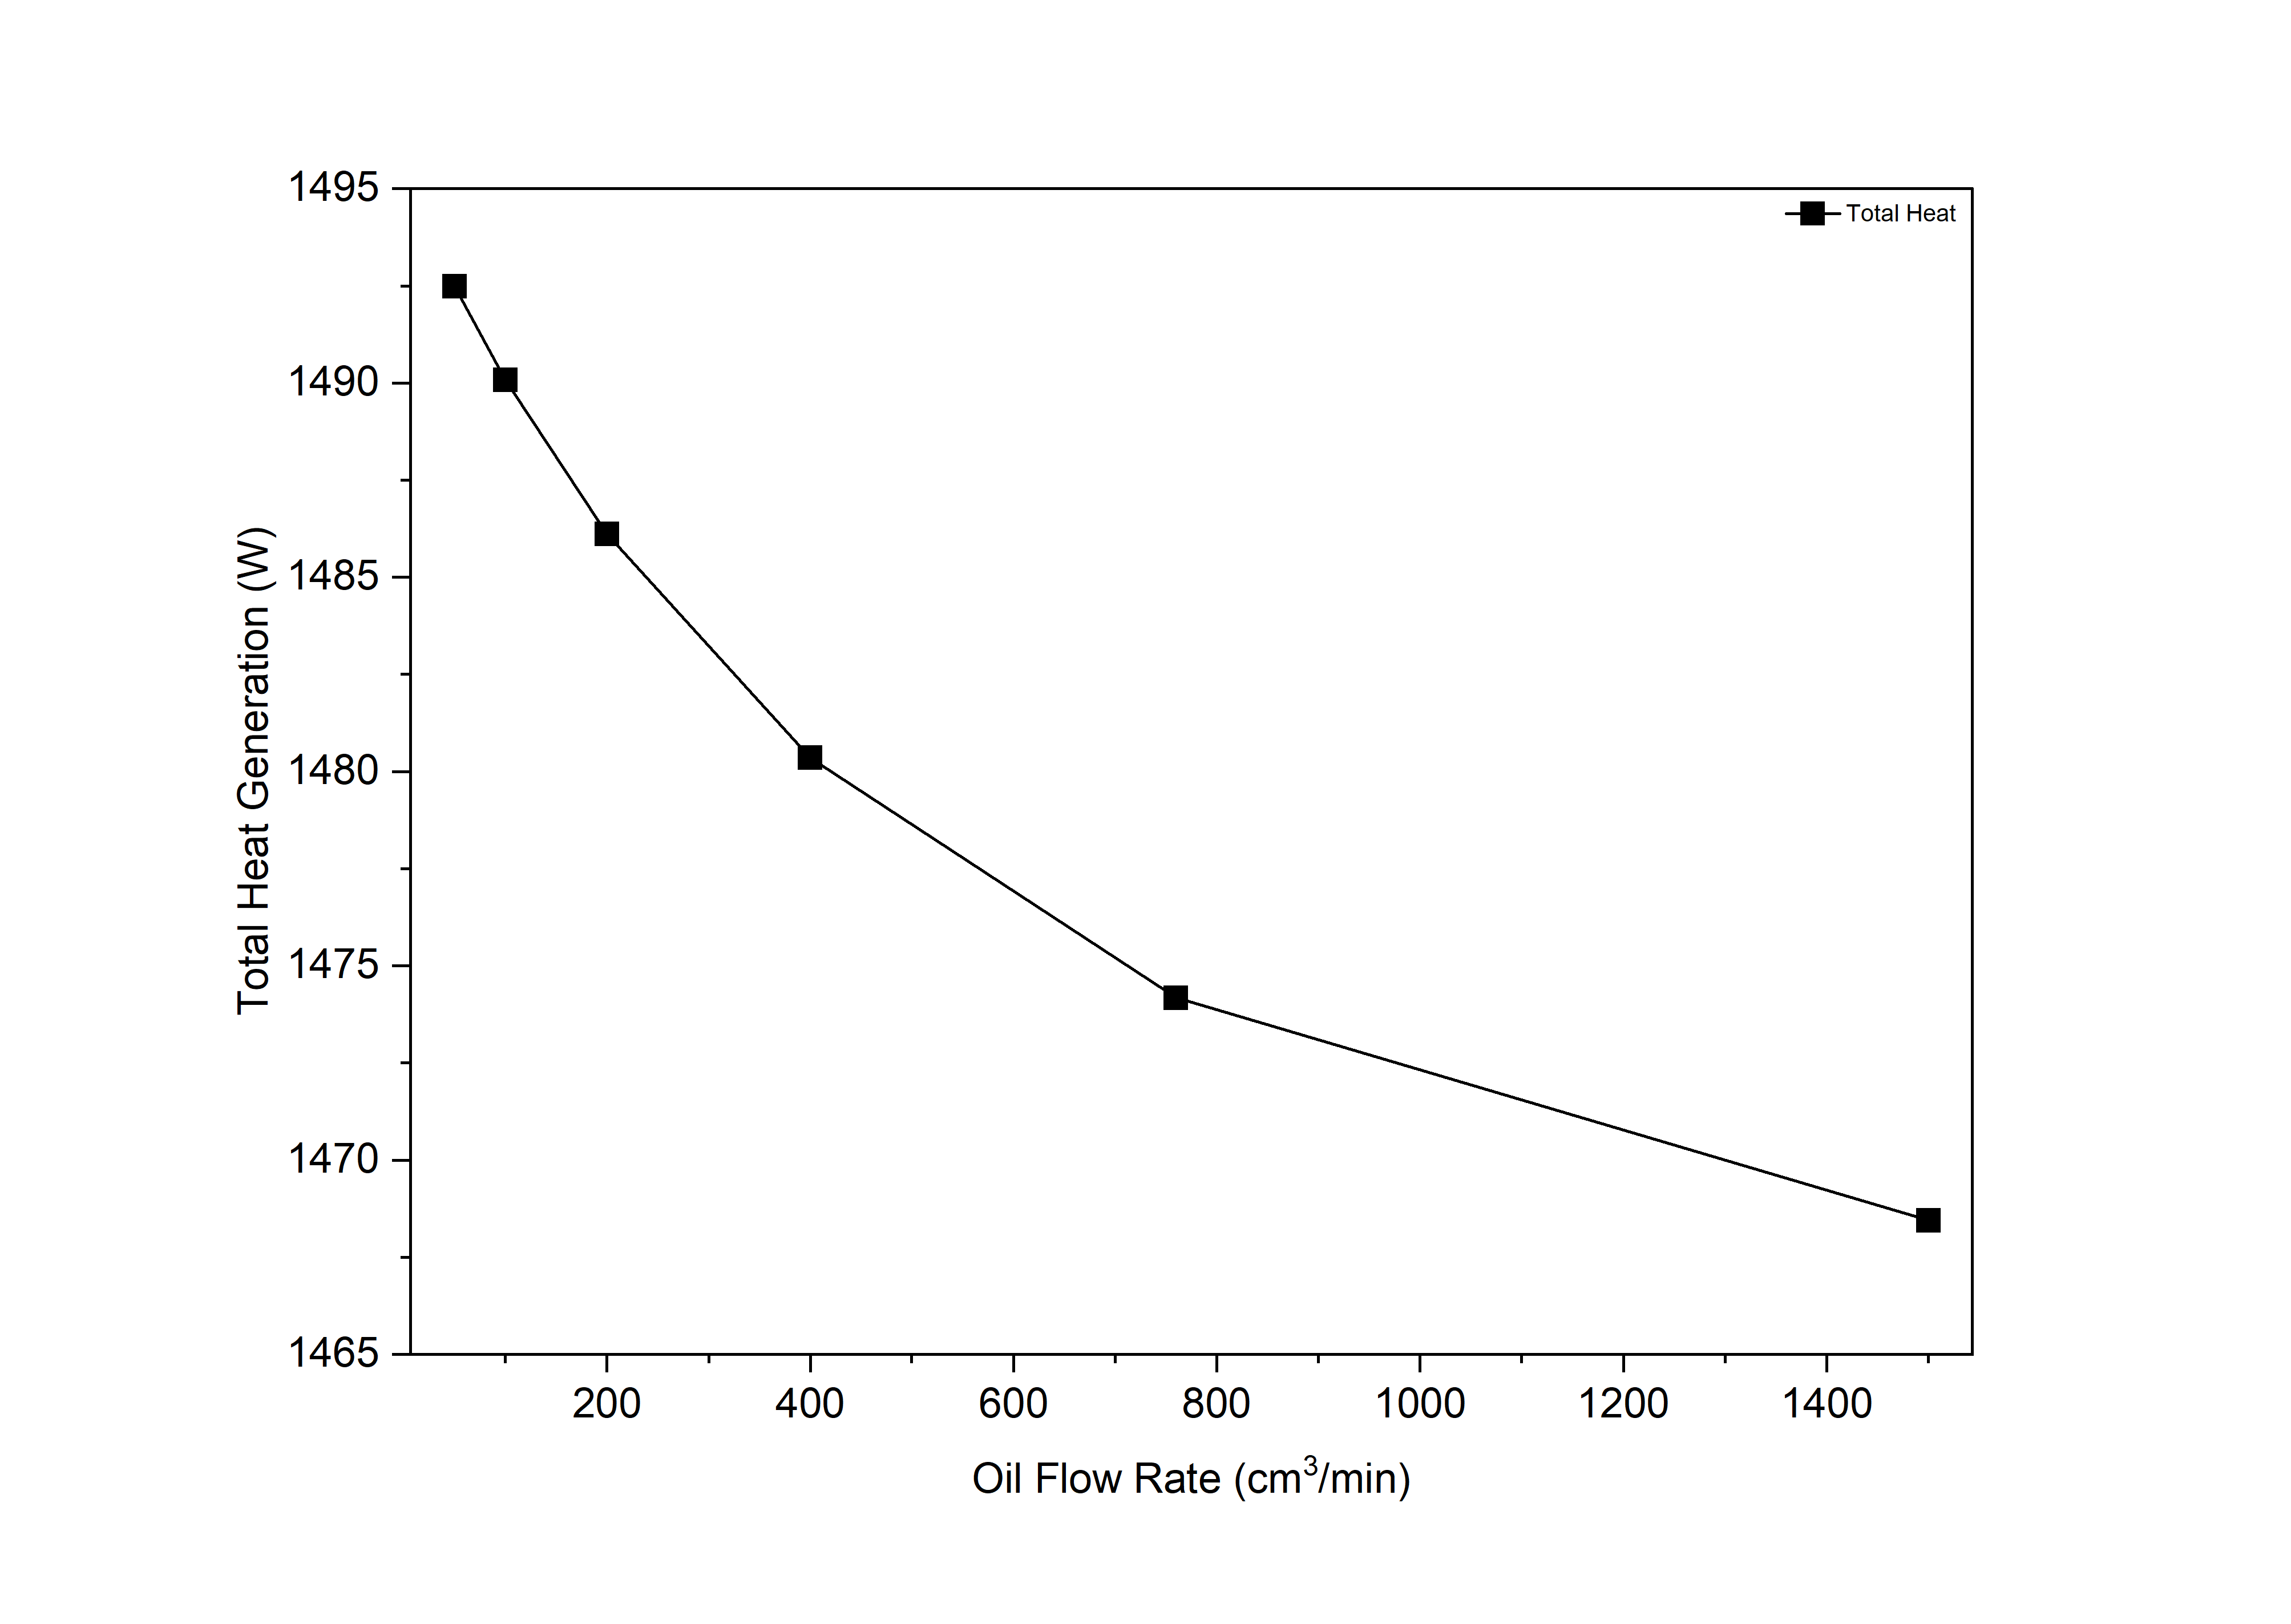
\includegraphics[width=12.0cm]{figures/oilflow_heat_generation.png}
    \caption{Total heat generation vs.\ oil flow rate. Same conditions as Figure~\ref{fig:oilflow_temp}.\label{fig:oilflow_heat}}
\end{figure}

A notable feature of the results is that all temperatures \emph{increase slightly} with increasing oil flow rate. At first glance, this appears counter-intuitive; however, it is a direct consequence of the high oil inlet temperature ($T_{\text{oil,in}} = 394$~K) being close to or above the oil sump equilibrium temperature. From Equation~(\ref{eq:oil_cooling}), the circulation cooling term $\dot{m}c_p(T_{\text{oil}} - T_{\text{oil,in}})$ is negative when $T_{\text{oil}} < T_{\text{oil,in}}$, meaning that fresh oil actually \emph{adds} thermal energy to the sump. At low flow rates, the oil sump finds a lower equilibrium ($\sim$384~K via ambient loss alone); increasing flow pushes $T_{\text{oil}}$ toward $T_{\text{oil,in}} = 394$~K, raising all component temperatures via the thermal network.

This observation is practically important: in systems where the oil is recirculated through a heat exchanger, the \emph{inlet temperature} is a far more effective control variable than the volume flow rate. The results indicate that, for this bearing and speed, reducing $T_{\text{oil,in}}$ by 10~K would lower bearing temperatures more than doubling the flow rate.


\subsection{Diametral Clearance Analysis}
\label{sec:clearance}

\subsubsection{Heavy Axial Preload ($F_a = 667$~N)}

The initial diametral clearance $P_d$ is swept over six values: 0, 5, 10, 15, 20, and 30~$\mu$m under the NASA baseline axial preload.

\begin{figure}[H]
    \centering
    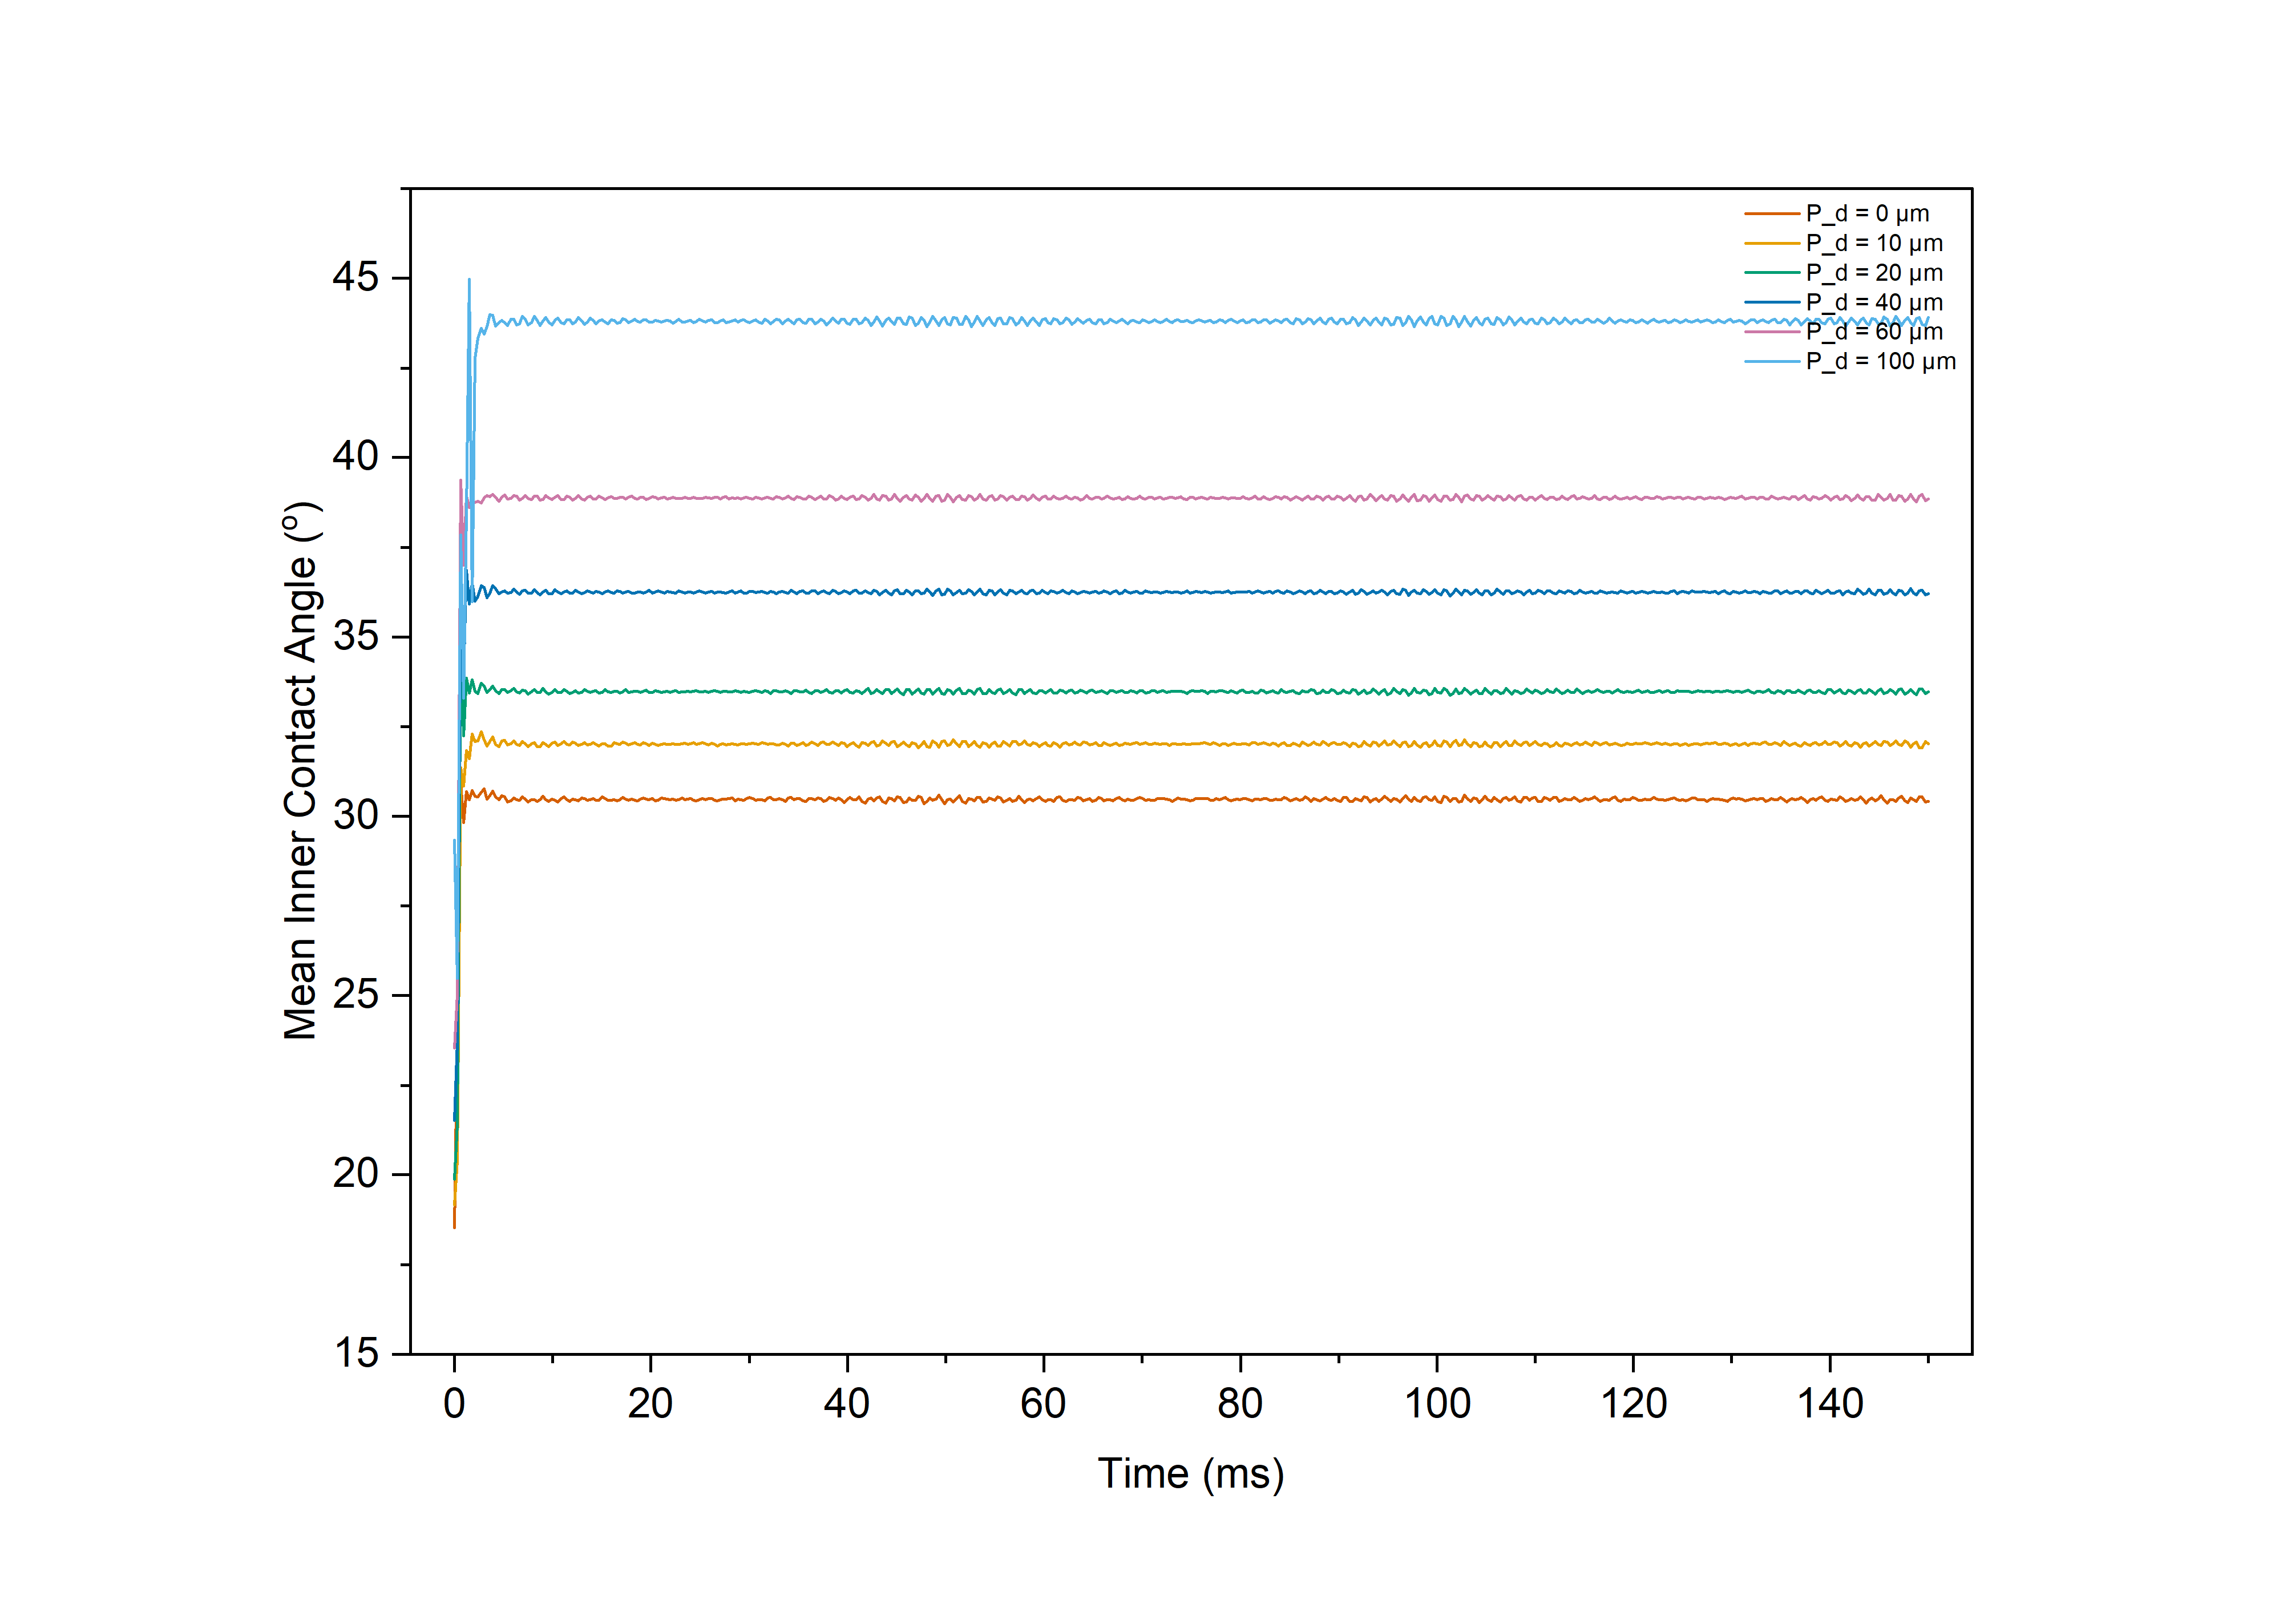
\includegraphics[width=12.0cm]{figures/clearance_transient_overlay.png}
    \caption{Transient inner race temperature for different initial diametral clearances (50,000~RPM, $F_a = 667$~N, $T_{\text{oil,in}} = 394$~K). All six curves overlap within $\pm 0.01$~K.\label{fig:clearance_transient}}
\end{figure}

\begin{figure}[H]
    \centering
    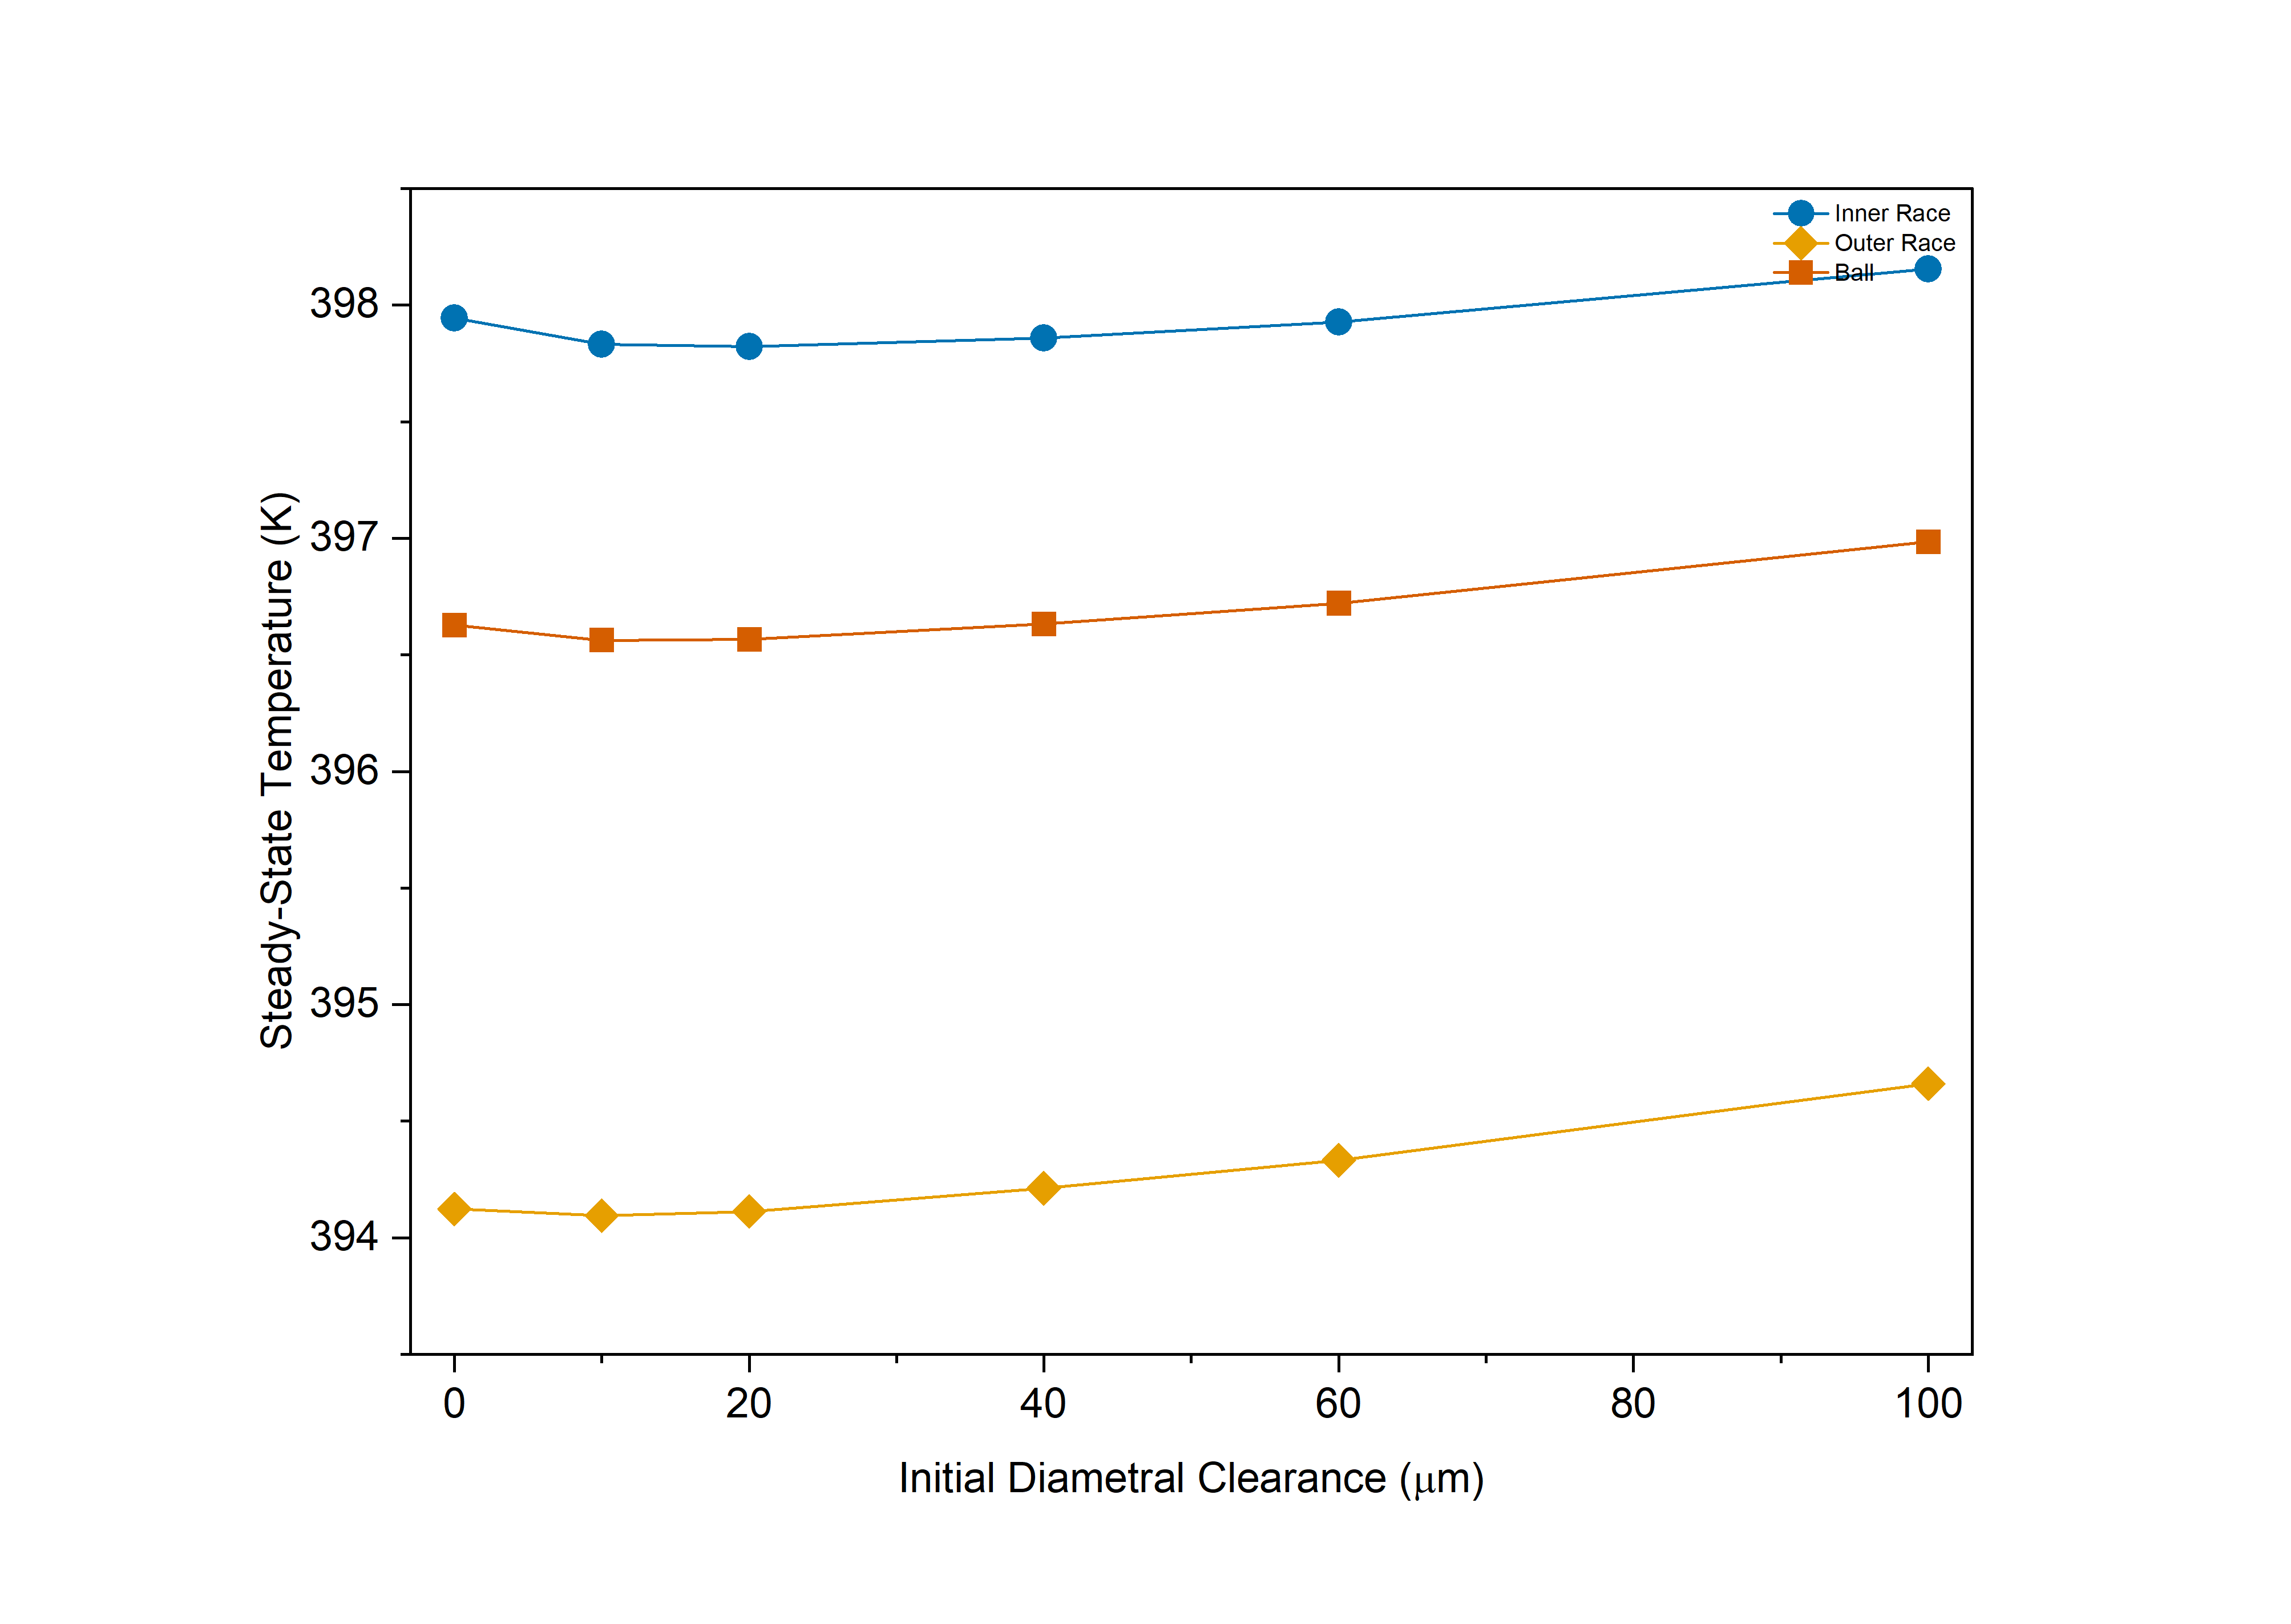
\includegraphics[width=14.0cm]{figures/clearance_steadystate.png}
    \caption{Steady-state temperature (left) and total heat generation (right) vs.\ initial diametral clearance.\label{fig:clearance_ss}}
\end{figure}

Within the present model formulation, no measurable thermal sensitivity to the tested clearance range (0--30~$\mu$m) was observed under the heavy axial preload condition. All six cases converge to identical steady-state temperatures and heat generation within numerical precision.

Under a 667~N axial thrust, the bearing operates in a fully preloaded regime: all 16~balls are in contact at all times, the contact angles adjust to accommodate the load regardless of initial clearance, and the resulting load distribution and sliding velocities are virtually identical across the clearance range. The 0--30~$\mu$m initial diametral clearance variation is smaller than the axial displacement imposed by the 667~N load ($\delta_a \approx 20$--40~$\mu$m). Furthermore, evaluating Equation~(\ref{eq:clearance_eff}) at 50,000~RPM quantitatively shows that inner race centrifugal expansion is on the order of $\approx 10$--15~$\mu$m, and thermal expansions for the races ($\delta r_{\text{IR}}, \delta r_{\text{OR}}$) are approximately 20--25~$\mu$m. These dynamic displacements combine with the axial deflection to comprehensively consume the initial clearance play.

\subsubsection{Combined Loading ($F_a = 100$~N, $F_r = 500$~N)}

To test whether clearance sensitivity emerges under a more demanding loading scenario, the sweep was repeated with combined loading ($F_a = 100$~N, $F_r = 500$~N) and an extended clearance range of 0--100~$\mu$m. Table~\ref{tab:clearance_combined} presents the results.

\begin{table}[H]
    \caption{Clearance sweep under combined loading ($F_a = 100$~N, $F_r = 500$~N, 50,000~RPM).\label{tab:clearance_combined}}
    \begin{tabularx}{\textwidth}{CCCCCC}
        \toprule
        \textbf{$P_d$ ($\mu$m)} & \textbf{$T_{\text{IR}}$ (K)} & \textbf{$T_{\text{OR}}$ (K)} & \textbf{$T_{\text{ball}}$ (K)} & \textbf{$H_{\text{total}}$ (W)} & \textbf{$\alpha_i$ ($^\circ$)} \\
        \midrule
        0 & 397.9 & 394.1 & 396.6 & 972 & 30.4 \\
        10 & 397.8 & 394.1 & 396.6 & 970 & 32.0 \\
        20 & 397.8 & 394.1 & 396.6 & 971 & 33.5 \\
        40 & 397.9 & 394.2 & 396.6 & 973 & 36.2 \\
        60 & 397.9 & 394.3 & 396.7 & 976 & 38.8 \\
        100 & 398.2 & 394.7 & 397.0 & 983 & 43.9 \\
        \bottomrule
    \end{tabularx}
\end{table}

Although the free contact angle responds strongly to clearance---increasing from $30.4^\circ$ at $P_d = 0$ to $43.9^\circ$ at $P_d = 100$~$\mu$m, in agreement with the Harris contact angle formula~\cite{Harris2006}---the thermal response remains minimal: $\Delta T_{\text{IR}} \approx 0.3$~K and $\Delta H_{\text{total}} \approx 12$~W (1.2\%) over the full 0--100~$\mu$m range. This result demonstrates that, within the present model, changes in contact angle caused by clearance are offset by adjustments in the load distribution and sliding velocity, producing nearly self-compensating thermal behavior.

\subsubsection{Model Diagnostic Interpretation}

\textbf{Model limitation}: the clearance insensitivity reported here should be interpreted as a diagnostic observation within the present model structure, not as a universal physical conclusion. Two structural factors contribute: (a)~the four-node LPTN averages all ball temperatures, making it unable to resolve circumferential heat distribution shifts caused by partial load zones (see Section~\ref{sec:lptn_limit}); and (b)~under preloaded conditions, the Hertzian contact stiffness dominates the equilibrium geometry such that clearance-induced contact angle changes are thermally compensated by the sliding velocity redistribution. Bossmanns and Tu~\cite{Bossmanns1999} demonstrated measurable clearance--temperature coupling in motorized spindle bearings using circumferentially resolved finite-element thermal models. The present LPTN, which assigns a single temperature to all rolling elements, is structurally unable to reproduce such effects. Different behavior would be expected under (i)~light preload with partial contact, (ii)~larger clearances ($> 100~\mu$m), or (iii)~a circumferentially resolved thermal network.


\subsection{Load Direction Effect}
\label{sec:loadratio}

The load direction is varied by rotating the resultant load vector $\bm{P}$ (magnitude $|\bm{P}| = 1000$~N) from nearly pure radial ($\theta = 10^\circ$) to pure axial ($\theta = 90^\circ$), where $F_a = |\bm{P}|\sin\theta$ and $F_r = |\bm{P}|\cos\theta$.

\begin{figure}[H]
    \centering
    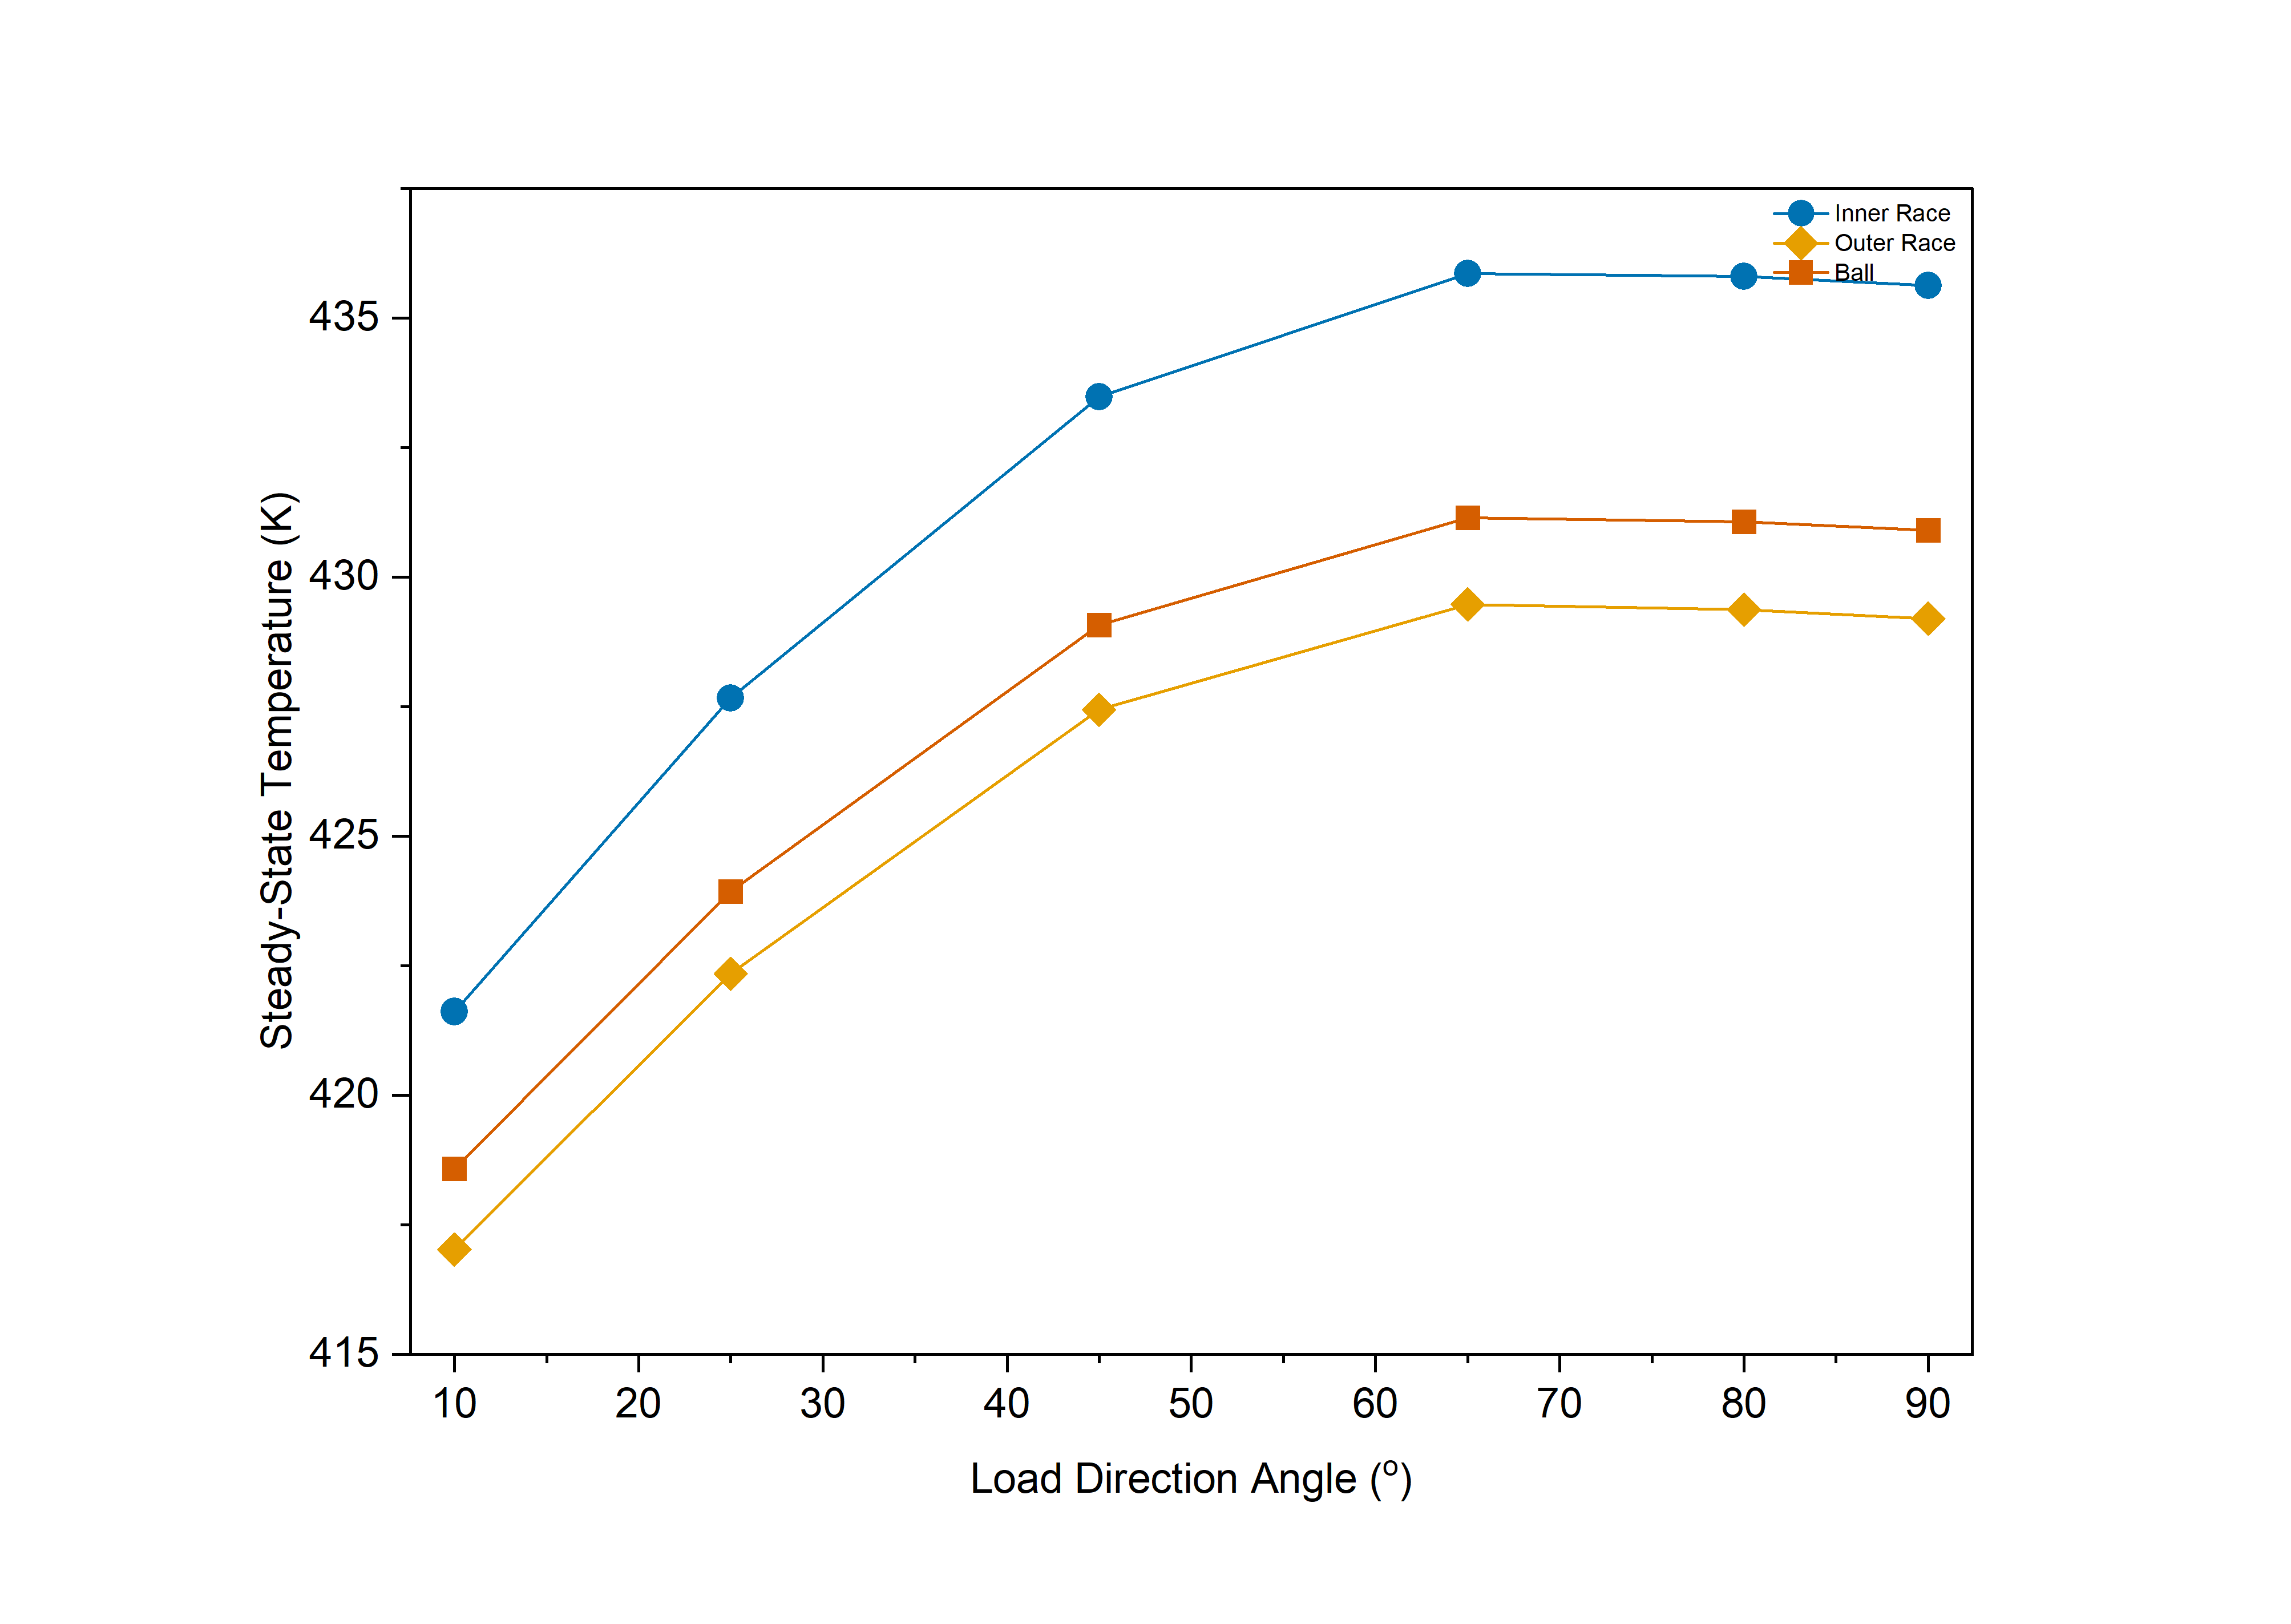
\includegraphics[width=14.0cm]{figures/loadratio_temperature.png}
    \caption{(\textbf{Left}) Steady-state temperatures vs.\ load angle $\theta$ ($|\bm{P}|= 1000$~N, 50,000~RPM, $T_{\text{oil,in}} = 394$~K). (\textbf{Right}) Inner--outer race temperature differential.\label{fig:loadratio_temp}}
\end{figure}

\begin{figure}[H]
    \centering
    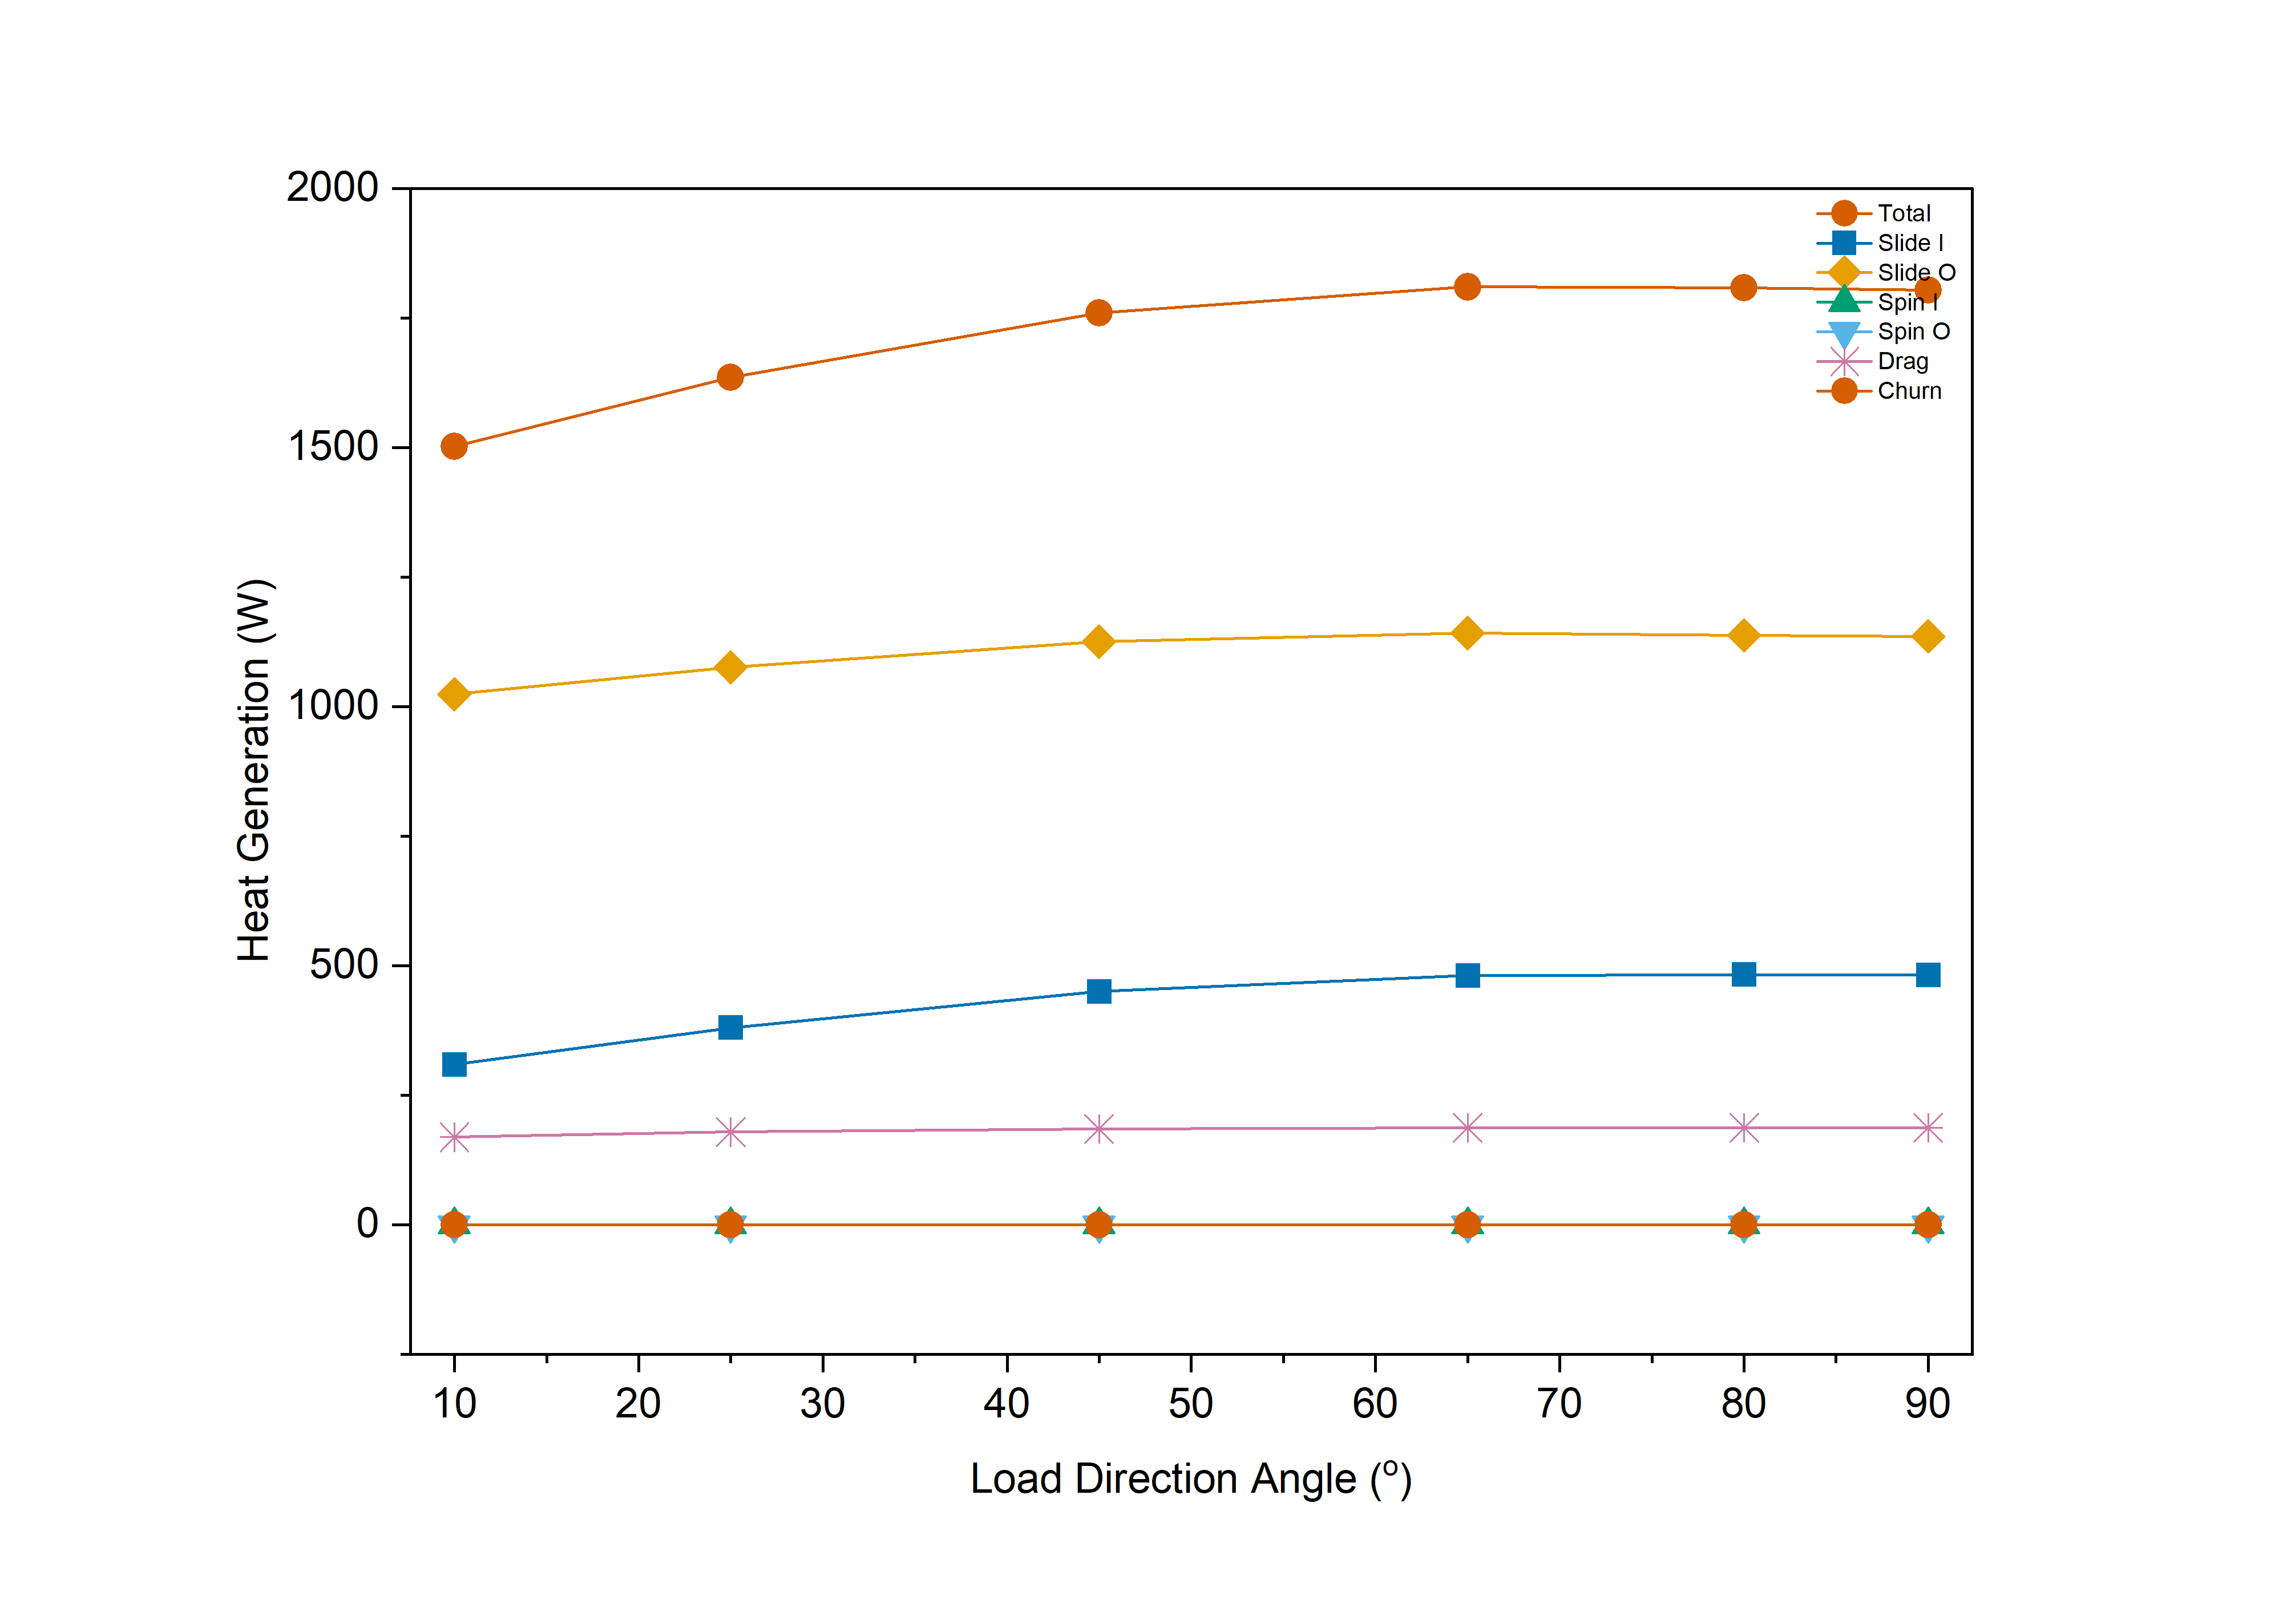
\includegraphics[width=12.0cm]{figures/loadratio_heat_breakdown.png}
    \caption{Heat source breakdown vs.\ load angle, showing all seven individual contributions. To ensure visual distinguishability in print, note that outer race sliding ($H_{\text{slide,o}}$, top portion) dominates over inner race sliding ($H_{\text{slide,i}}$), followed by macroscopic translational drag ($H_{\text{drag}}$). The spin components ($H_{\text{spin,i}}$, $H_{\text{spin,o}}$) and churning ($H_{\text{churn}}$) are negligibly small under the present operating conditions (see text). Conditions: same as Figure~\ref{fig:loadratio_temp}.\label{fig:loadratio_heat}}
\end{figure}

Table~\ref{tab:loadratio} presents the numerical results.

\begin{table}[H]
    \caption{Load direction parametric study results ($|\bm{P}| = 1000$~N, 50,000~RPM).\label{tab:loadratio}}
    \begin{tabularx}{\textwidth}{CCCCCCC}
        \toprule
        \textbf{$\theta$} & \textbf{$F_a$} & \textbf{$F_r$} & \textbf{$T_{\text{IR}}$} & \textbf{$\Delta T_{\text{IR-OR}}$} & \textbf{$H_{\text{total}}$} & \textbf{$H_{\text{slide,o}}/H_{\text{total}}$} \\
        & (N) & (N) & (K) & (K) & (W) & (\%) \\
        \midrule
        10$^\circ$ & 174 & 985 & 394.5 & 4.9 & 651 & 62 \\
        25$^\circ$ & 423 & 906 & 397.5 & 5.5 & 709 & 59 \\
        45$^\circ$ & 707 & 707 & 403.2 & 6.4 & 811 & 55 \\
        65$^\circ$ & 906 & 423 & 407.1 & 7.0 & 872 & 54 \\
        80$^\circ$ & 985 & 174 & 408.7 & 7.3 & 895 & 53 \\
        90$^\circ$ & 1000 & 0 & 409.0 & 7.3 & 900 & 53 \\
        \bottomrule
    \end{tabularx}
\end{table}

The load direction has a pronounced effect on thermal behavior:
\begin{itemize}
    \item Inner race temperature increases by 15~K from $\theta = 10^\circ$ to $90^\circ$.
    \item The inner--outer race differential increases by 50\% ($4.9 \to 7.3$~K).
    \item Total heat generation increases by 38\% ($651 \to 900$~W).
    \item Outer race sliding friction ($H_{\text{slide,o}}$) dominates total heat generation across all load angles, contributing 53--62\%. Its fraction decreases with increasing axial load as inner race sliding grows.
    \item Inner race spinning ($H_{\text{spin,i}}$) is negligibly small ($< 0.01$~W) because the gyroscopic spin moment at the inner contact is resisted almost entirely by the outer contact. Churning heat ($H_{\text{churn}}$) is likewise negligible due to the very low oil fill fraction ($\phi = 0.002$) and the small ball radius, which keep the effective mixture density---and thus the drag torque---near zero (see Section~\ref{sec:scope}).
\end{itemize}


%% ======================================================================
\section{Discussion}
\label{sec:discussion}

\subsection{Mechanistic Interpretation}

The load-direction results (Table~\ref{tab:loadratio}) can be explained through the contact mechanics: under pure axial load ($\theta = 90^\circ$), all 16 balls carry equal loads but at a higher contact angle ($\alpha > \alpha_0$), increasing the gyroscopic moment and spin-induced micro-slip. The increased inner race sliding friction ($H_{\text{slide,i}}$ from 125~W to 263~W) arises because the inner race surface velocity $v_{\text{IR}} = \omega_{\text{IR}} \cdot r_{\text{contact}}$ increases with the higher effective contact radius at the elevated contact angle. Notably, the heat breakdown (Figure~\ref{fig:loadratio_heat}) reveals that sliding friction at the two raceways accounts for $> 95\%$ of total heat generation at all load angles, with translational cage drag providing the remainder ($\approx$~100--160~W). The inner and outer race spinning moments, as well as churning, contribute negligibly under these conditions; the former because gyroscopic spin is predominantly resisted at the outer race, and the latter because the under-race jet lubrication yields an extremely low cavity fill fraction ($\phi = 0.002$).

Under predominantly radial loading ($\theta = 10^\circ$), fewer balls in the loaded zone carry concentrated loads, but the overall friction is lower because the reduced axial preload decreases the net normal load and contact stress.

\subsection{Oil Flow Rate Paradox}

The counter-intuitive oil flow result (Section~\ref{sec:oilflow}) is a consequence of the specific operating conditions: $T_{\text{oil,in}} = 394$~K is relatively high (near the ball temperature), and the oil sump reaches a lower equilibrium via ambient losses alone. In applications with cooler inlet oil ($T_{\text{oil,in}} < T_{\text{sump,eq}}$), the conventional trend (higher flow $\to$ lower temperature) would be recovered. This finding highlights the importance of reporting oil inlet temperature in thermal studies.

\subsection{Comparison with Literature}

The predicted temperature ranking ($T_{\text{ball}} > T_{\text{IR}} > T_{\text{OR}} > T_{\text{oil}}$) and the inner--outer race differential of 5--8~K are consistent with the experimental observations of Takabi and Khonsari~\cite{Takabi2013}, who measured outer race temperature rises of 5--15~K above inlet for similar DN values. The temperature rise magnitudes are within the same order, although direct comparison is limited by differences in bearing geometry and lubrication method.

\subsection{Cross-Bearing Size Limitation}
\label{sec:cross}

To assess the model's generalization beyond the validated 35-mm reference bearing, the same model (with geometry updated to the 120-mm bore bearing from NASA TP-2275) was applied without re-tuning any traction or network parameters. The predictions systematically under-predicted heat generation by approximately $3\times$ at 5,000--12,000~RPM. This offset is attributed to: (i)~increased churning losses in larger bearings due to higher oil volume fractions, (ii)~size-dependent traction scaling, and (iii)~different thermal boundary conditions for a housed 120-mm bearing.

\subsection{Scope and Limitations}
\label{sec:scope}

Therefore, the validated operational envelope for the current specific churning and traction parameter set is restricted to:
\begin{itemize}
    \item The NASA 35-mm bore ACBB geometry (Table~\ref{tab:geometry}) and similar high-speed, small-to-medium bore bearings.
    \item The high-speed DN range of $1.0$--$2.5 \times 10^6$.
    \item The MIL-L-23699 lubricant properties (Table~\ref{tab:lubricant}).
    \item The thermal network parameters in Table~\ref{tab:thermal}, which carry an inherent uncertainty of $\pm 10$--$30$~K in absolute temperature (Section~\ref{sec:gij_sensitivity}).
\end{itemize}

Extension to other bearing sizes, lubricant types, or DN ranges would require re-validation of the churning model and thermal conductance values. The 120-mm cross-prediction demonstrates that direct extrapolation without re-calibration leads to significant errors.


%% ======================================================================
\section{Conclusions}
\label{sec:conclusion}

A transient multi-physics simulation framework, validated against NASA TP-2275 experimental heat generation data (6.0\% mean absolute deviation, $\pm 3\%$ digitization uncertainty) and cross-checked against Palmgren/SKF friction torque correlations, was applied to investigate the thermal parametric sensitivities of a single 35-mm bore angular contact ball bearing at DN~$= 1.75 \times 10^6$. Three parametric studies led to the following findings, which apply specifically to this bearing configuration and model formulation:

\begin{enumerate}
    \item Under the tested conditions ($T_{\text{oil,in}} = 394$~K), increasing oil flow rate slightly increases bearing temperatures due to the warm-oil-in thermal coupling. This demonstrates that \emph{oil inlet temperature} is a more effective thermal control variable than volume flow rate when the inlet is near the sump equilibrium.

    \item Within the present model formulation, diametral clearance variations in the range 0--100~$\mu$m produced no detectable thermal effect under axial preload ($F_a = 100$--$667$~N). This observation reflects the model's treatment of clearance as an initial quasi-static parameter and the limitations of the four-node LPTN in resolving clearance-dependent load-zone effects.

    \item Shifting the load direction from near-radial ($10^\circ$) to pure axial ($90^\circ$) at constant resultant magnitude (1000~N) increases inner race temperature by 15~K and total heat generation by 38\%, driven by increased sliding and spin friction at higher contact angles.
\end{enumerate}

The traction and churning model coefficients used in this study are representative of the 35-mm bearing class and are not yet demonstrated to be universal across bearing sizes; the 120-mm cross-prediction (Section~\ref{sec:cross}) confirms that these parameters are size-dependent. Future work should extend these investigations to larger bearing sizes with re-calibrated churning models, explore the effect of lower oil inlet temperatures to recover the conventional flow--cooling relationship, and develop circumferentially resolved thermal networks to properly capture clearance-dependent load-zone effects.


%%%%%%%%%%%%%%%%%%%%%%%%%%%%%%%%%%%%%%%%%%
\authorcontributions{Conceptualization, methodology, software, validation, formal analysis, investigation, data curation, writing---original draft preparation, visualization, Y.L. The author has read and agreed to the published version of the manuscript.}

\funding{This research received no external funding.}

\institutionalreview{Not applicable.}

\informedconsent{Not applicable.}

\dataavailability{The simulation framework, all input configuration files, and post-processing scripts used in this study are available at \url{https://github.com/YUXinluhk/BallBearing-Dynamics} (release v1.0). A README with step-by-step reproduction instructions is included.}

\conflictsofinterest{The author declares no conflicts of interest.}

%%%%%%%%%%%%%%%%%%%%%%%%%%%%%%%%%%%%%%%%%%
\abbreviations{Abbreviations}{
The following abbreviations are used in this manuscript:
\\

\noindent
\begin{tabular}{@{}ll}
ACBB & Angular contact ball bearing\\
CTE & Coefficient of thermal expansion\\
DOF & Degree of freedom\\
EHL & Elasto-hydrodynamic lubrication\\
FBDF & Fixed-leading-coefficient backward differentiation formula\\
LPTN & Lumped-parameter thermal network
\end{tabular}
}

%%%%%%%%%%%%%%%%%%%%%%%%%%%%%%%%%%%%%%%%%%
\begin{adjustwidth}{-\extralength}{0cm}

\reftitle{References}

\isAPAandChicago{}{%
\begin{thebibliography}{999}

\bibitem[Harris and Kotzalas(2006)]{Harris2006}
Harris, T.A.; Kotzalas, M.N. \textit{Rolling Bearing Analysis}, 5th ed.; CRC Press: Boca Raton, FL, USA, 2006.

\bibitem[Takabi and Khonsari(2013)]{Takabi2013}
Takabi, J.; Khonsari, M.M. Experimental testing and thermal analysis of ball bearings. {\em Tribol. Int.} {\bf 2013}, {\em 60}, 93--103.

\bibitem[Parker(1984)]{Parker1984}
Parker, R.J. Comparison of predicted and experimental thermal performance of angular-contact ball bearings. NASA Technical Paper 2275, 1984.

\bibitem[Palmgren(1959)]{Palmgren1959}
Palmgren, A. \textit{Ball and Roller Bearing Engineering}, 3rd ed.; Burbank: Philadelphia, PA, USA, 1959.

\bibitem[SKF(2018)]{SKF2018}
SKF Group. \textit{Rolling Bearings}; SKF Publication PUB BU/P1 10000/2 EN; SKF Group: Gothenburg, Sweden, 2018.

\bibitem[Gupta(1984)]{Gupta1984}
Gupta, P.K. \textit{Advanced Dynamics of Rolling Elements}; Springer: New York, NY, USA, 1984.

\bibitem[Stacke \textit{et al.}(1999)]{Stacke1999}
Stacke, L.E.; Fritzson, D.; Nordling, P. BEAST---A rolling bearing simulation tool. {\em Proc. Inst. Mech. Eng. Part K J. Multi-Body Dyn.} {\bf 1999}, {\em 213}, 63--71.

\bibitem[Jang and Jeong(2004)]{Jang2004}
Jang, G.; Jeong, S.W. Nonlinear excitation model of ball bearing waviness in a rigid rotor supported by two or more ball bearings considering five degrees of freedom. {\em ASME J. Tribol.} {\bf 2004}, {\em 126}, 82--90.

\bibitem[Bizarre \textit{et al.}(2018)]{Bizarre2018}
Bizarre, L.; Nonato, F.; Cavalca, K.L. Formulation of five degrees of freedom ball bearing model accounting for the nonlinear stiffness and damping of elastohydrodynamic point contacts. {\em Mech. Mach. Theory} {\bf 2018}, {\em 124}, 179--196.

\bibitem[Rackauckas and Nie(2017)]{Rackauckas2017}
Rackauckas, C.; Nie, Q. DifferentialEquations.jl---A performant and feature-rich ecosystem for solving differential equations in Julia. {\em J. Open Res. Softw.} {\bf 2017}, {\em 5}, 15.

\bibitem[Zheng \textit{et al.}(2018)]{Zheng2018}
Zheng, D.; Chen, W.; Li, M. An optimized thermal network model to estimate thermal performances on a pair of angular contact ball bearings under oil-air lubrication. {\em Appl. Therm. Eng.} {\bf 2018}, {\em 131}, 328--339.

\bibitem[Liu \textit{et al.}(2020)]{Liu2020}
Liu, J.; Shao, Y. Overview of dynamic modelling and analysis of rolling element bearings with localized and distributed faults. {\em Nonlinear Dyn.} {\bf 2020}, {\em 93}, 1765--1798.

\bibitem[Hamrock and Dowson(1977)]{Hamrock1977}
Hamrock, B.J.; Dowson, D. Isothermal elastohydrodynamic lubrication of point contacts: Part III---Fully flooded results. {\em ASME J. Lubr. Technol.} {\bf 1977}, {\em 99}, 264--276.

\bibitem[Bair and Winer(1979)]{Bair1979}
Bair, S.; Winer, W.O. A rheological model for elastohydrodynamic contacts based on the primary laboratory data. {\em ASME J. Lubr. Technol.} {\bf 1979}, {\em 101}, 258--265.

\bibitem[Zhang \textit{et al.}(2024)]{Zhang2024}
Zhang, X.; Wang, Y.; Li, C. Advanced thermal-fluid-solid coupling analysis of high-speed rolling bearings in electric vehicle powertrains. {\em Tribol. Int.} {\bf 2024}, {\em 192}, 109245.

\bibitem[Bossmanns and Tu(1999)]{Bossmanns1999}
Bossmanns, B.; Tu, J.F. A thermal model for high-speed motorized spindles. {\em Int. J. Mach. Tools Manuf.} {\bf 1999}, {\em 39}, 1345--1366.

\end{thebibliography}
}

\PublishersNote{}
\end{adjustwidth}
\end{document}
